\section{Программная реализация}

\subsection{Сервис векторизации текста (Embedding Model Service)}

\subsubsection{Класс модели эмбеддингов}

Центральным элементом сервиса является класс \texttt{EmbeddingModel}, реализующий интерфейс \texttt{Embeddings} из LangChain. Ключевой особенностью реализации является использование \textbf{семантических префиксов}: фрагменты документов векторизуются с префиксом \texttt{"passage: "}, а поисковые запросы — с префиксом \texttt{"query: "}. Это требование модели семейства \texttt{multilingual-e5}, обеспечивающее корректное сравнение векторов документов и запросов в едином пространстве. Реализация класса показана на рисунке \ref{code_1}.

\begin{figure}[H]
    \centering
    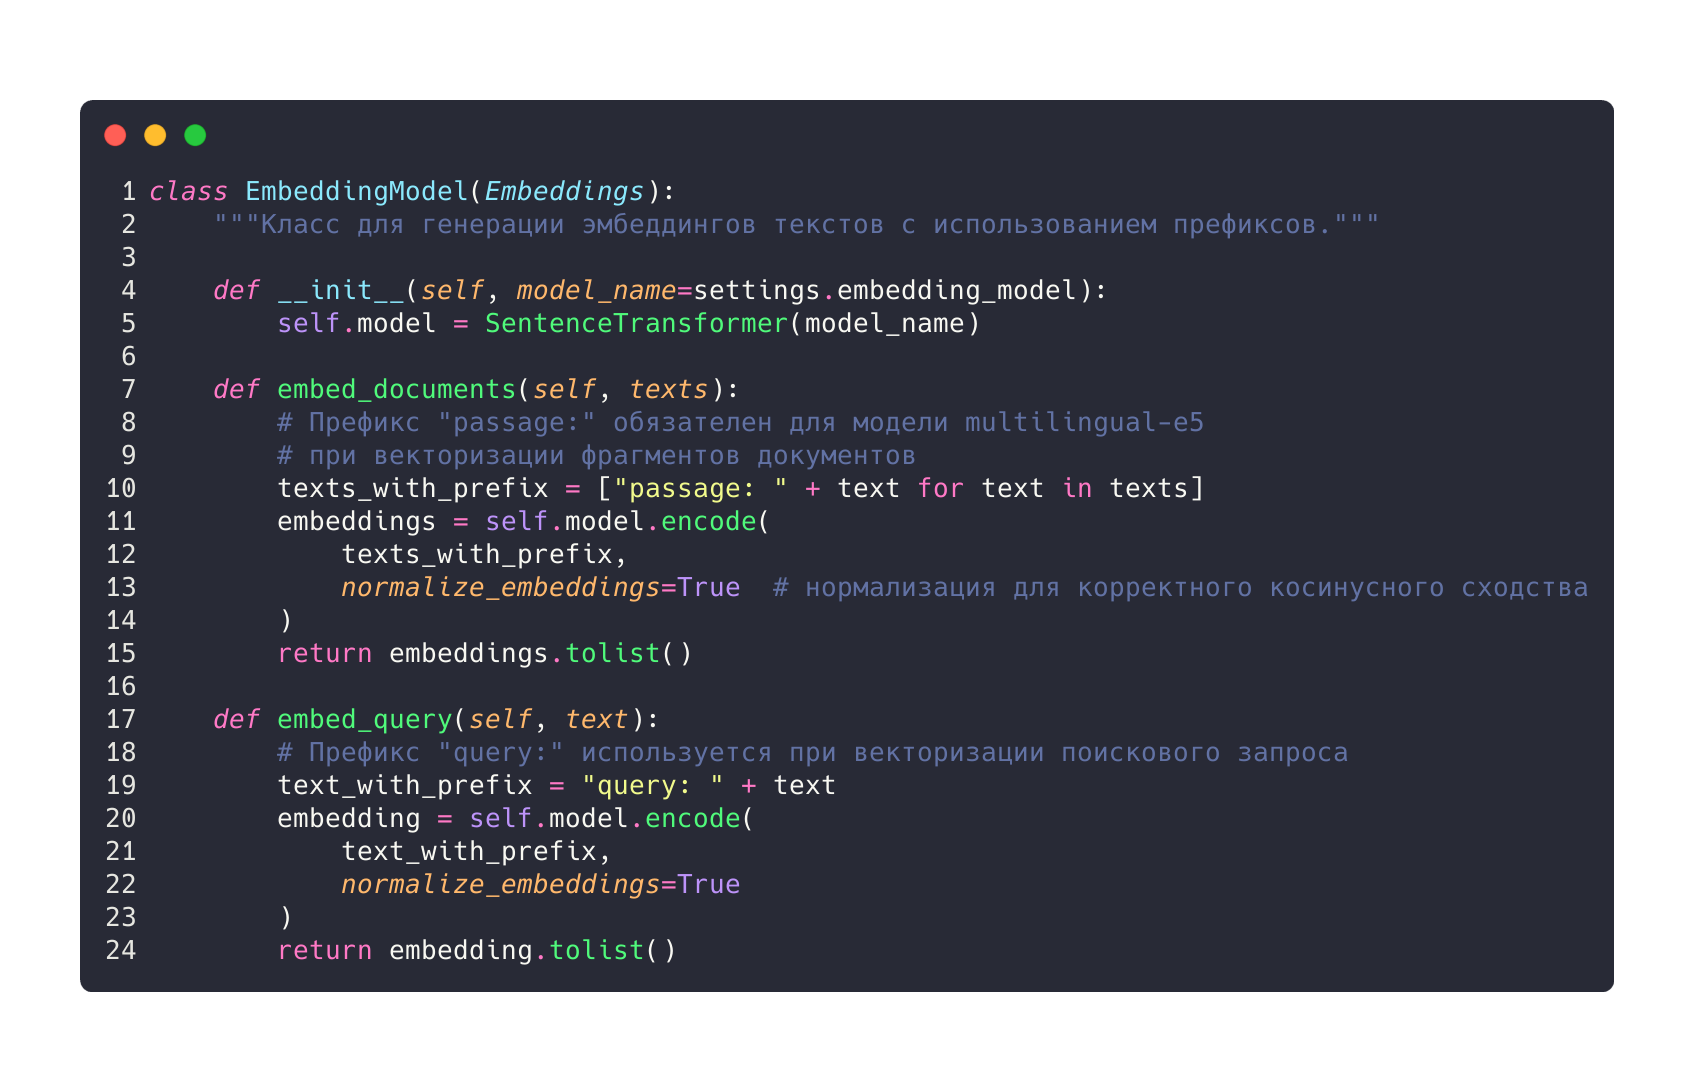
\includegraphics[width=\textwidth]{materials/codes/1.png}
    \caption{Реализация класса \texttt{EmbeddingModel} с использованием семантических префиксов}
    \label{code_1}
\end{figure}

\subsubsection{Инициализация сервиса и REST API}

Модель загружается в память единожды при старте приложения через механизм \texttt{lifespan} FastAPI и помещается в глобальный словарь \texttt{ml\_models}. Это исключает накладные расходы на повторную инициализацию при каждом запросе. Сервис предоставляет два раздельных эндпоинта: для векторизации батча документов и для векторизации одиночного поискового запроса. Инициализация модели и эндпоинты сервиса приведены на рисунке \ref{code_2}.

\begin{figure}[H]
    \centering
    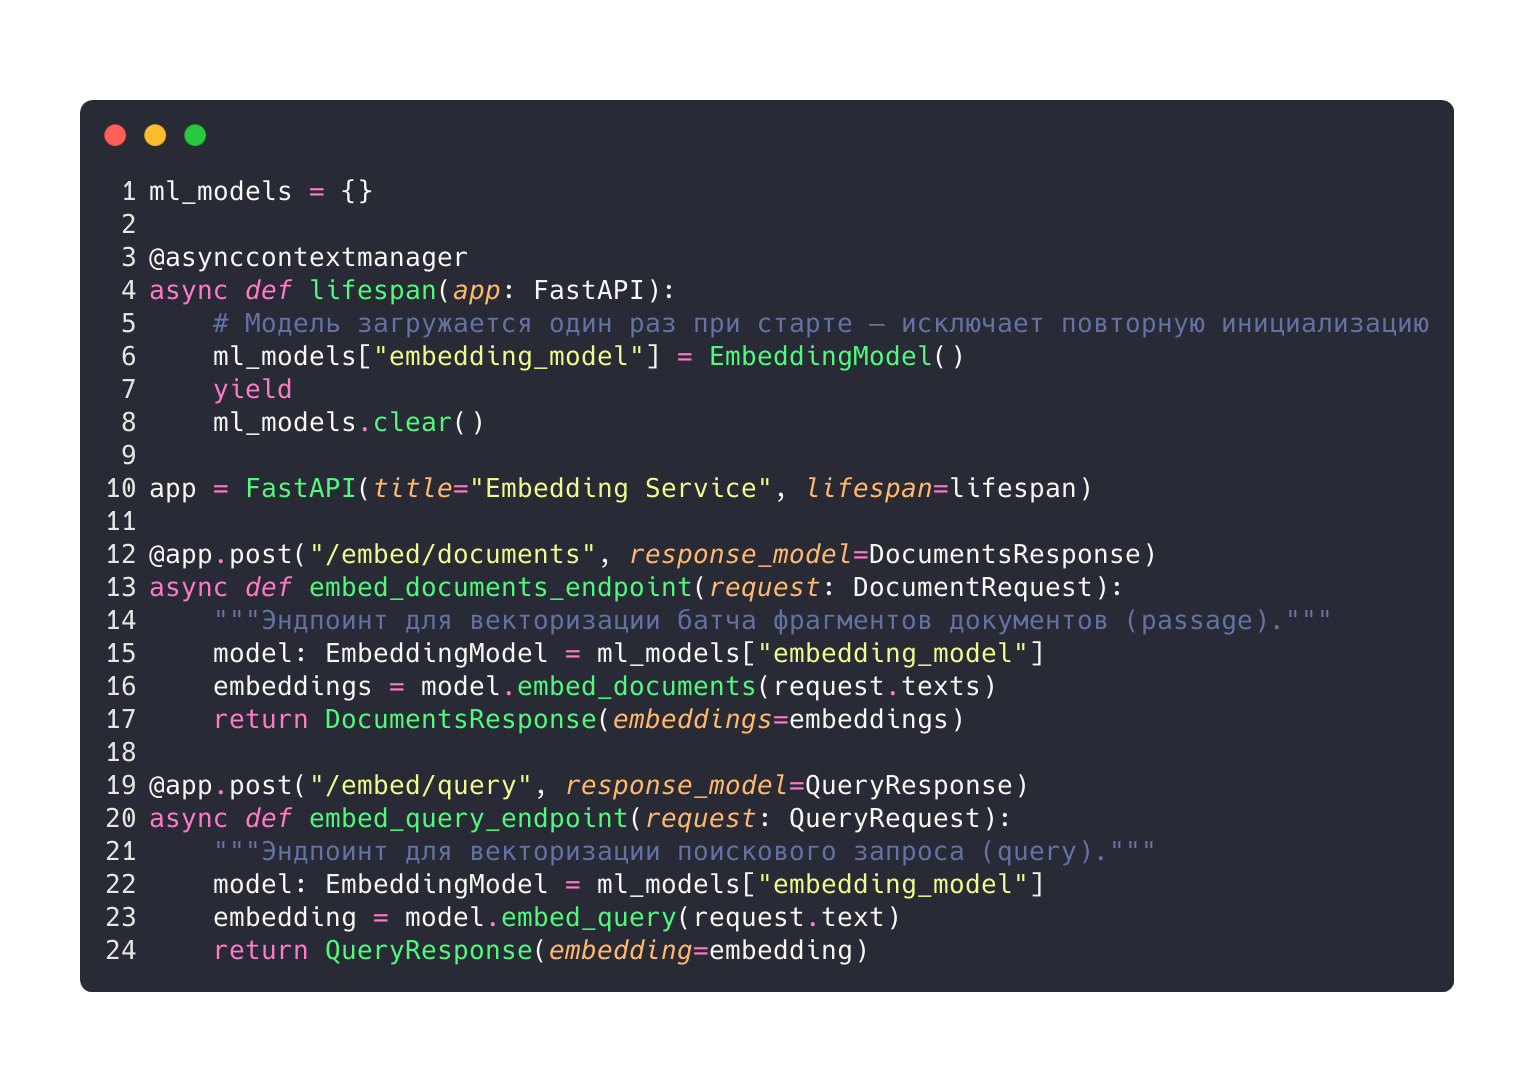
\includegraphics[width=\textwidth]{materials/codes/2.png}
    \caption{Инициализация модели через \texttt{lifespan} FastAPI и определение эндпоинтов векторизации}
    \label{code_2}
\end{figure}

\subsection{Конвейер индексации (Ingest Pipeline Service)}

\subsubsection{Приём запроса и постановка задачи в очередь}

API-эндпоинт принимает \texttt{file\_id} загруженного файла и незамедлительно ставит задачу его обработки в очередь Redis, возвращая пользователю \texttt{job\_id} для последующей проверки статуса. Тяжёлая обработка не блокирует HTTP-ответ. Реализация приема запроса показана на рисунке \ref{code_3}.

\begin{figure}[H]
    \centering
    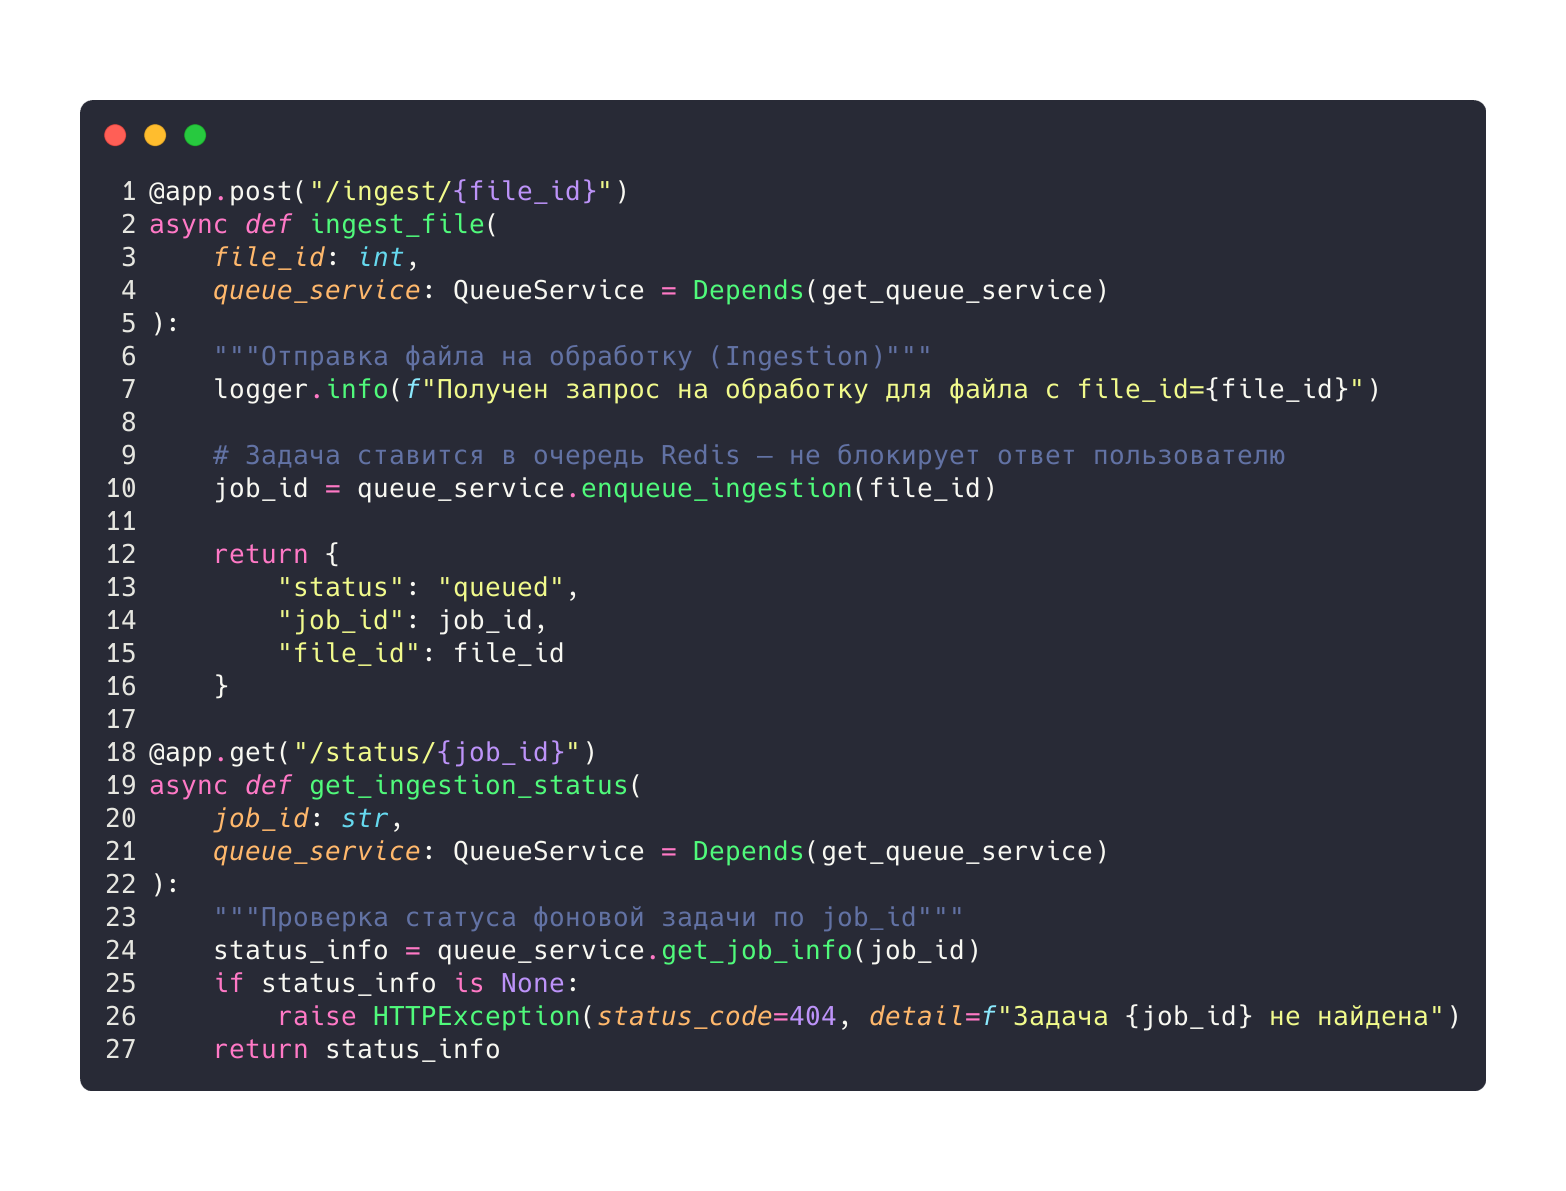
\includegraphics[width=\textwidth]{materials/codes/3.png}
    \caption{API-эндпоинт приёма \texttt{file\_id} и постановки задачи в очередь Redis}
    \label{code_3}
\end{figure}

\subsubsection{Сервис управления очередью задач}

\texttt{QueueService} инкапсулирует работу с Redis Queue: постановку задач на обработку и получение их текущего статуса. Название очереди \texttt{"ingestion"} совпадает с именем очереди, которую слушает воркер. Сервис управления очередью приведен на рисунке \ref{code_4}.

\begin{figure}[H]
    \centering
    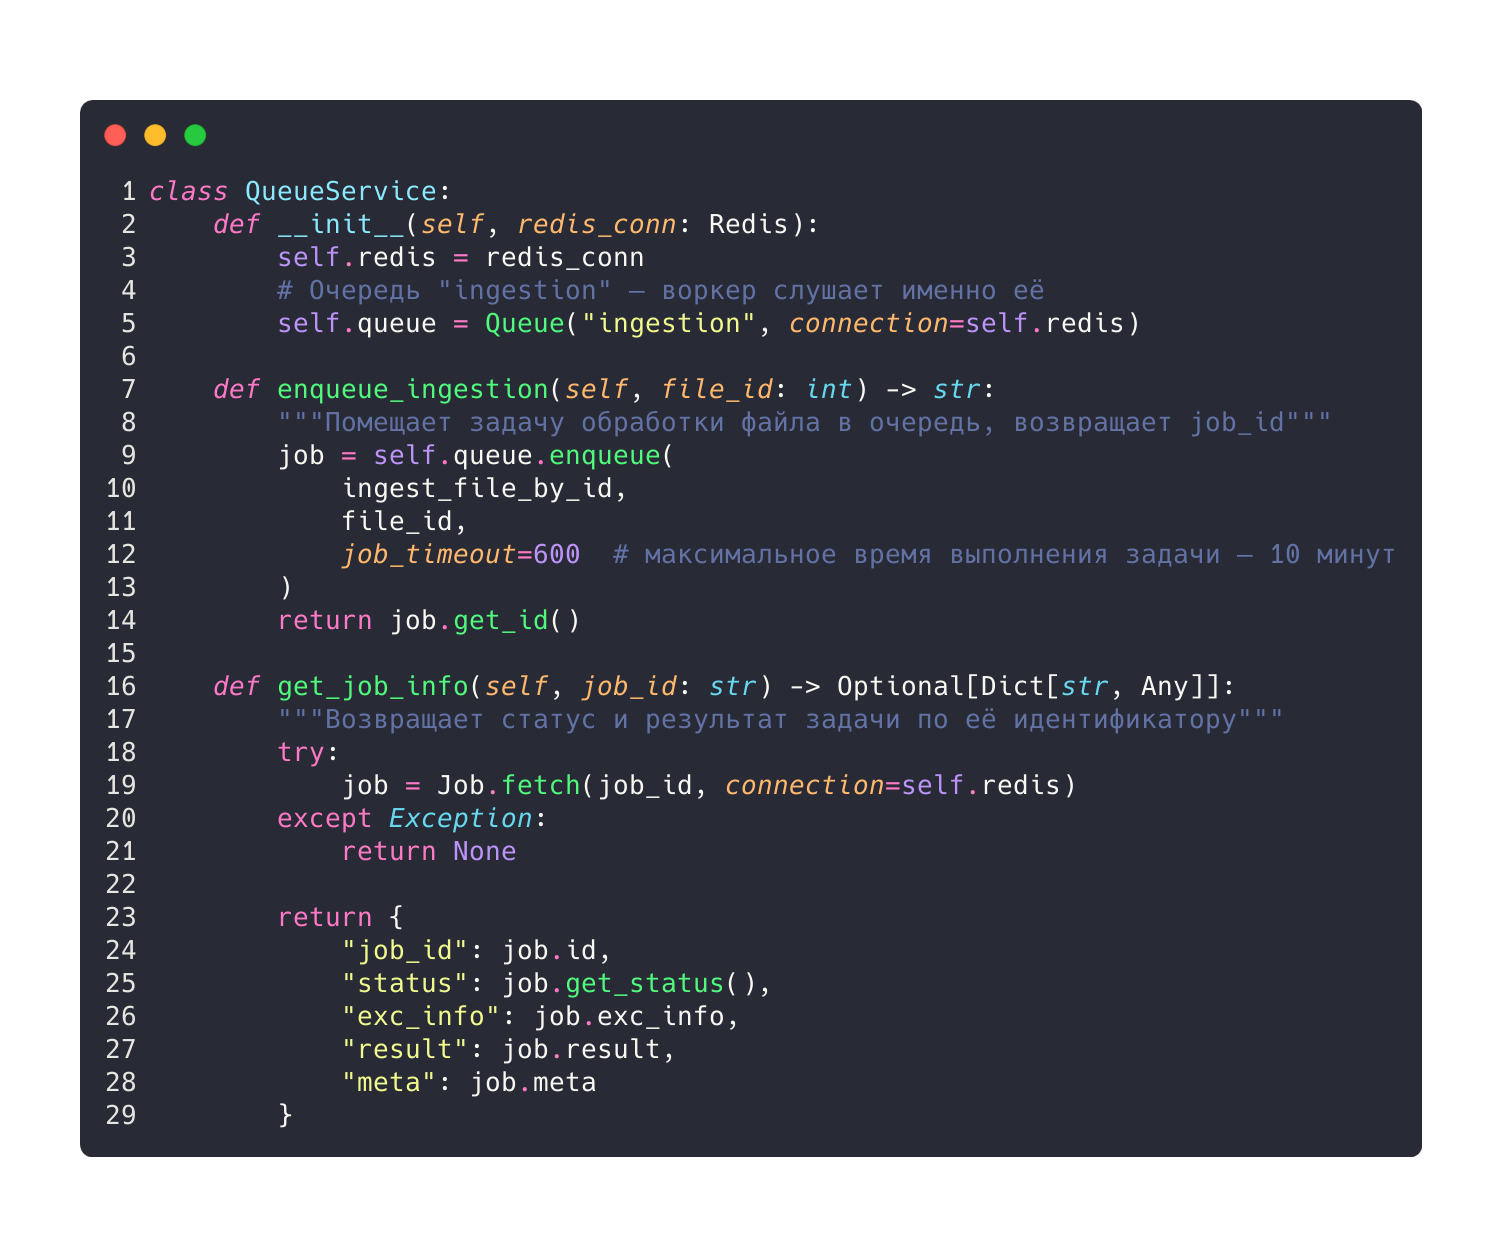
\includegraphics[width=\textwidth]{materials/codes/4.png}
    \caption{Сервис \texttt{QueueService} для работы с Redis Queue}
    \label{code_4}
\end{figure}

\subsubsection{Запуск фонового воркера}

Воркер запускается как отдельный процесс и непрерывно обрабатывает задачи из очереди \texttt{"ingestion"}. Запуск фонового воркера показан на рисунке \ref{code_5}.

\begin{figure}[H]
    \centering
    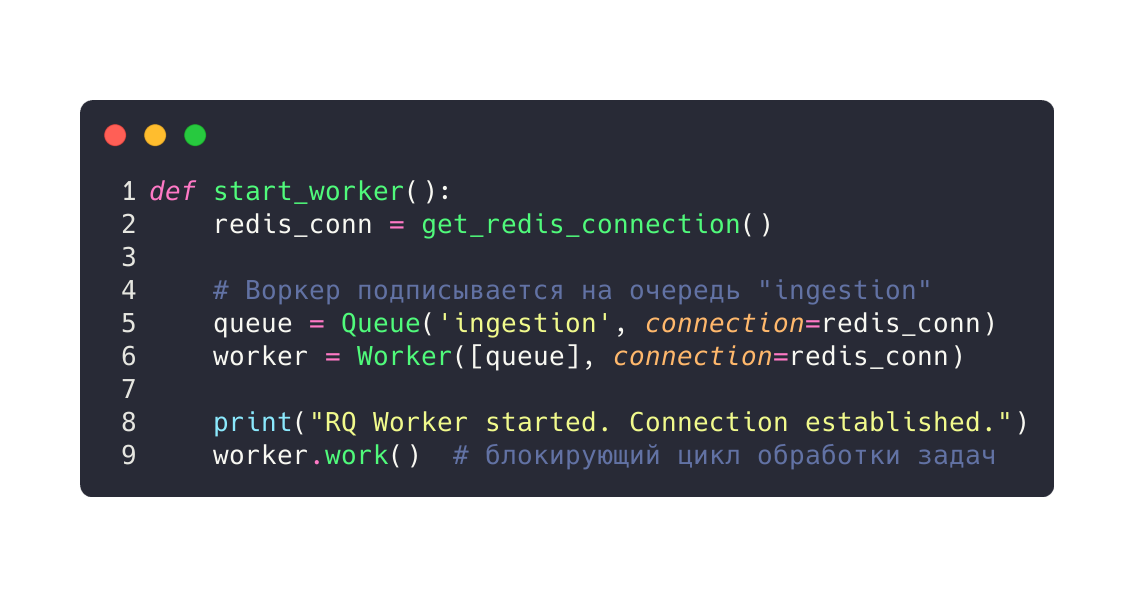
\includegraphics[width=\textwidth]{materials/codes/5.png}
    \caption{Запуск фонового воркера, обрабатывающего очередь \texttt{ingestion}}
    \label{code_5}
\end{figure}

\subsubsection{Сервис векторизации и сохранения в ChromaDB}

\texttt{VectorService} в контексте ingest-пайплайна отвечает за получение эмбеддингов от Embedding Model Service и сохранение пар (текст чанка, вектор, метаданные) в ChromaDB. Коллекция ChromaDB создаётся лениво при первом обращении с метрикой косинусного сходства. Метод сохранения эмбеддингов показан на рисунке \ref{code_6}.

\begin{figure}[H]
    \centering
    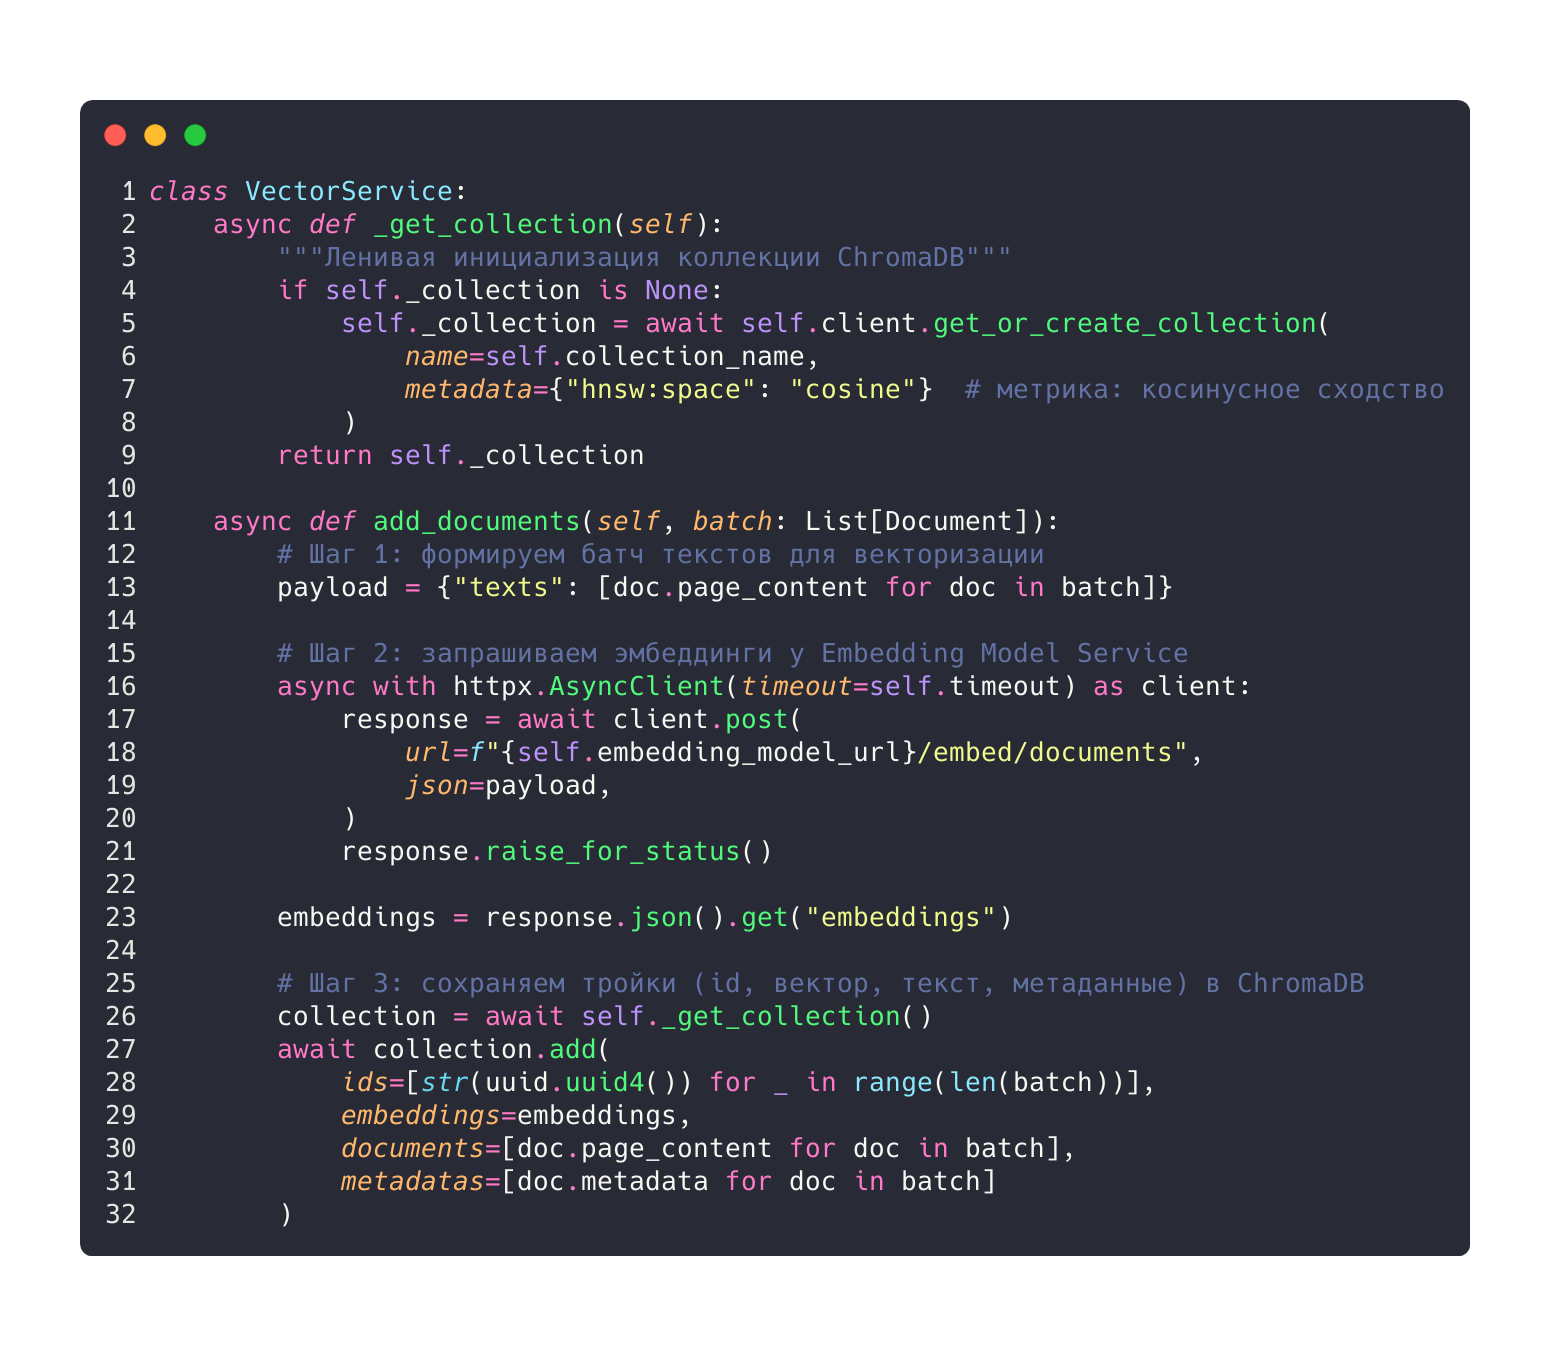
\includegraphics[width=\textwidth]{materials/codes/6.png}
    \caption{Метод \texttt{VectorService} для получения эмбеддингов и сохранения в ChromaDB}
    \label{code_6}
\end{figure}

\subsubsection{Загрузка файла из MinIO во временное хранилище}

Перед обработкой воркер скачивает файл из объектного хранилища MinIO во временную директорию \texttt{.tmp} для последующего парсинга. Загрузка файла из MinIO приведена на рисунке \ref{code_7}.

\begin{figure}[H]
    \centering
    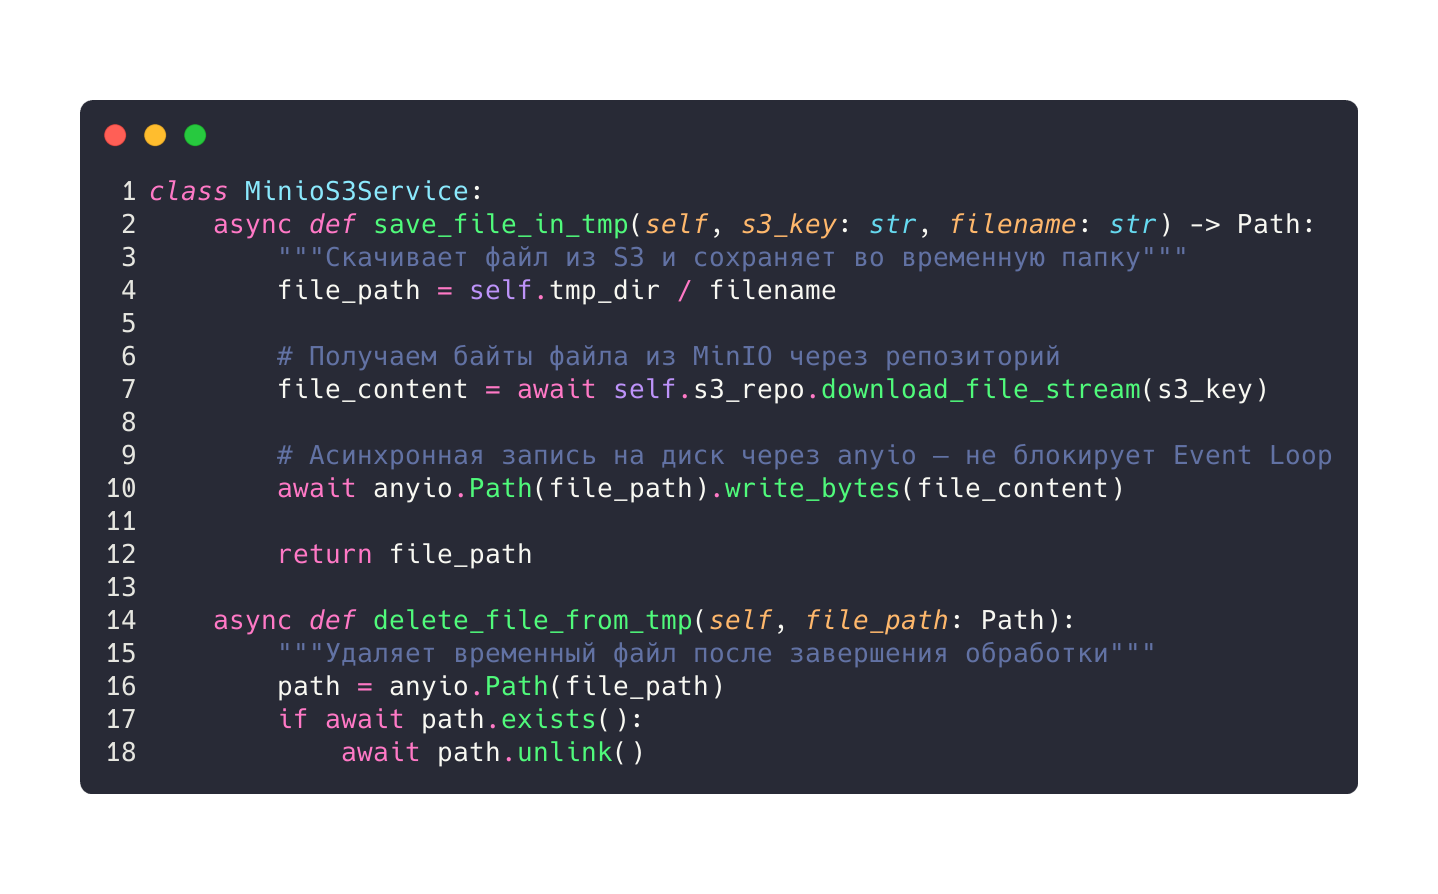
\includegraphics[width=\textwidth]{materials/codes/7.png}
    \caption{Загрузка файла из MinIO во временную директорию \texttt{.tmp}}
    \label{code_7}
\end{figure}

\subsection{Конвейер поиска (Retrieval Pipeline Service)}

\texttt{VectorService} в retrieval-пайплайне выполняет семантический поиск: векторизует запрос пользователя через Embedding Model Service и выполняет поиск Top-K ближайших векторов в ChromaDB по косинусному расстоянию. Метод семантического поиска показан на рисунке \ref{code_8}.

\begin{figure}[H]
    \centering
    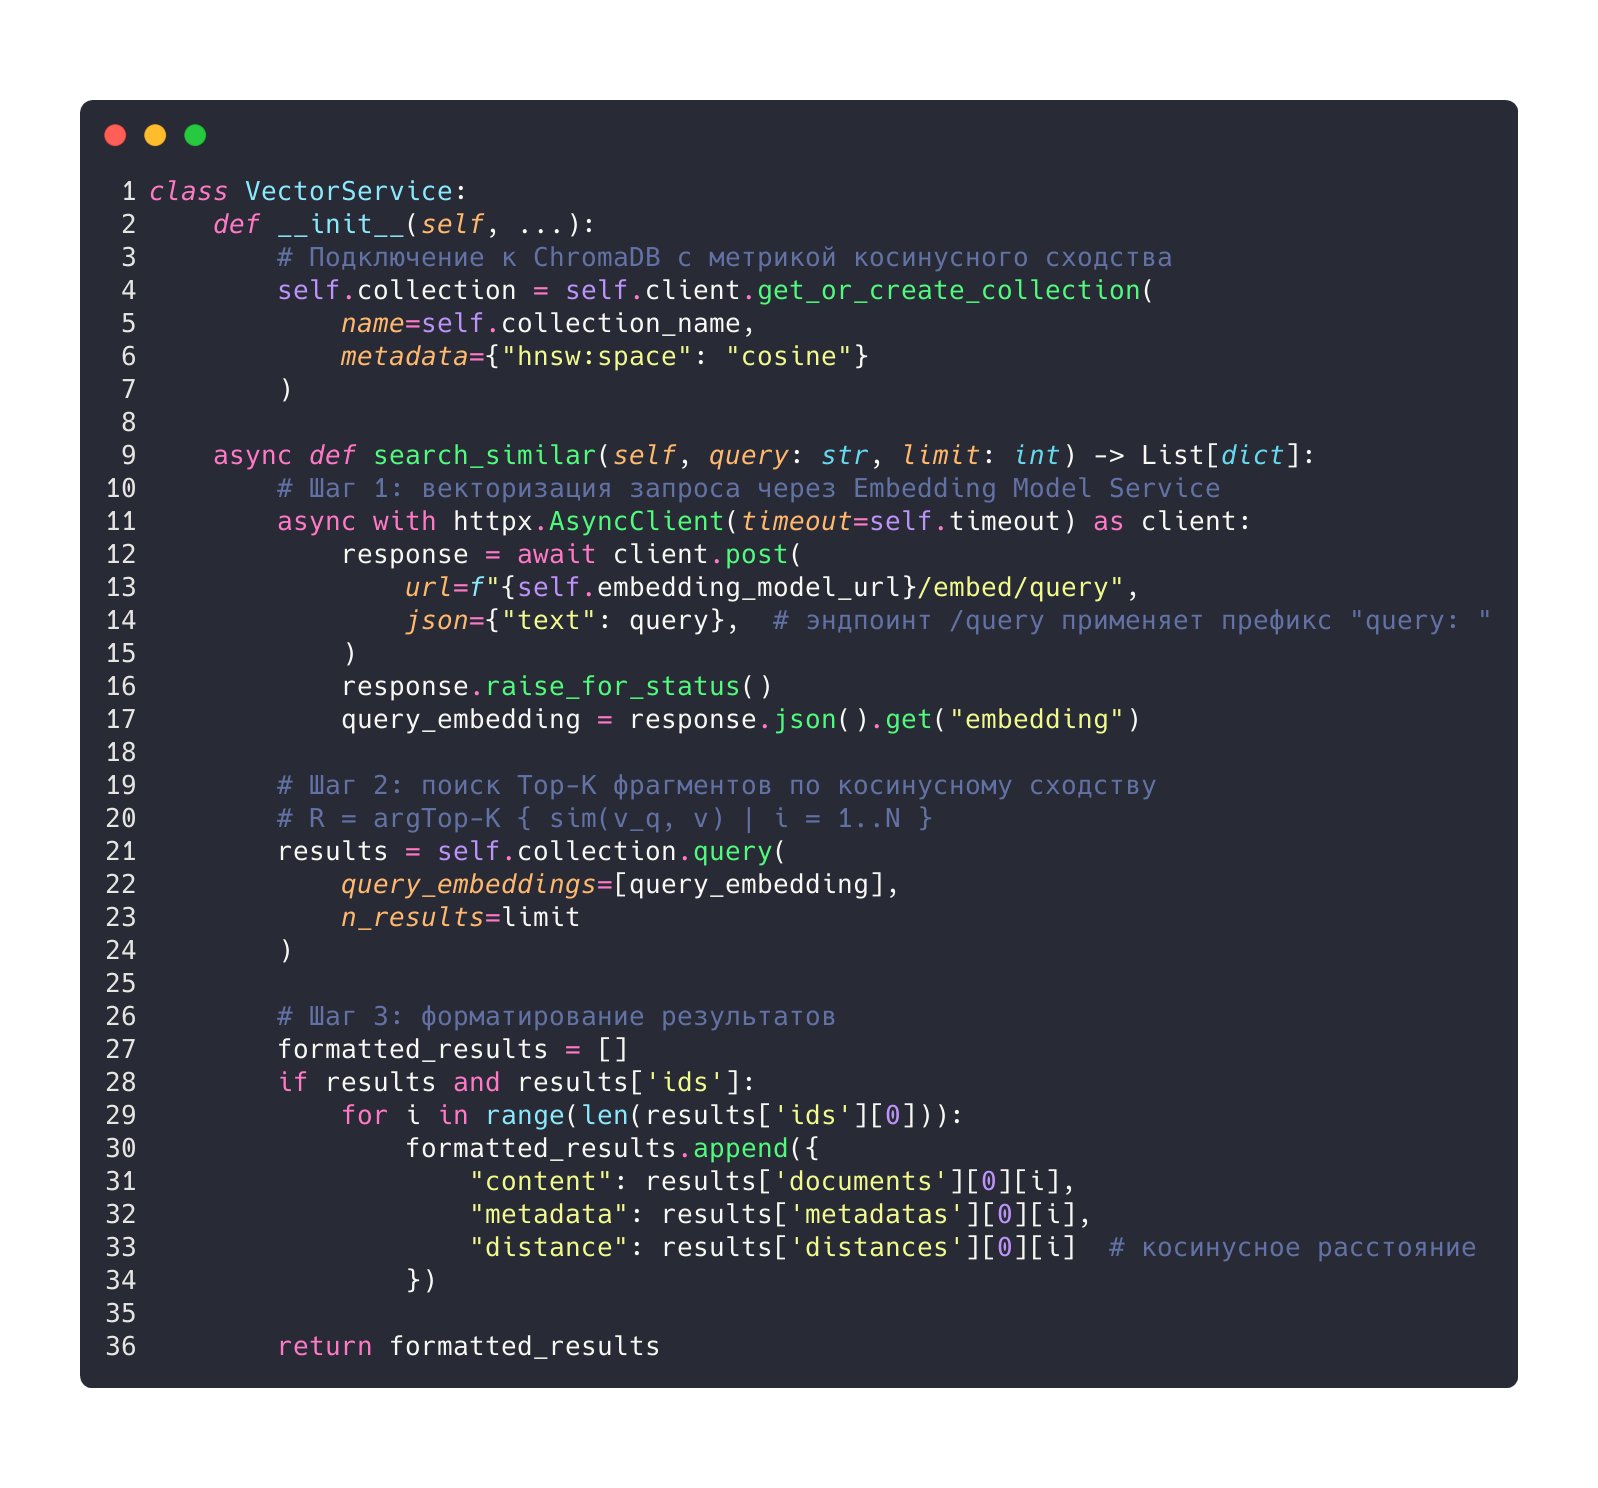
\includegraphics[width=\textwidth]{materials/codes/8.png}
    \caption{Метод семантического поиска в \texttt{VectorService} для retrieval-пайплайна}
    \label{code_8}
\end{figure}

Эндпоинт сервиса, принимающий запрос и возвращающий список релевантных фрагментов, приведен на рисунке \ref{code_9}.

\begin{figure}[H]
    \centering
    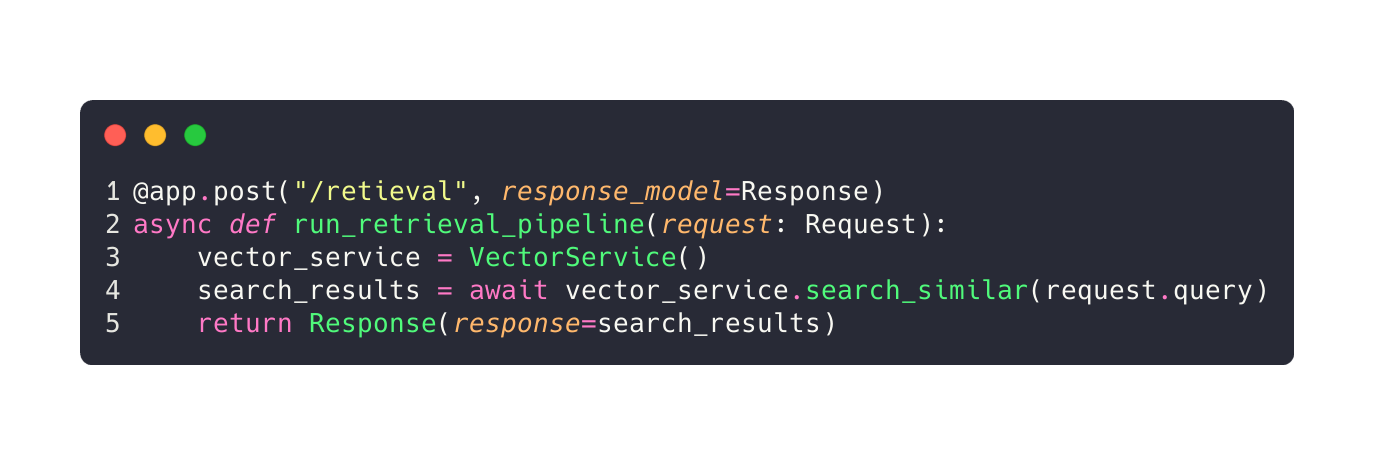
\includegraphics[width=\textwidth]{materials/codes/9.png}
    \caption{Эндпоинт retrieval-сервиса для поиска релевантных фрагментов}
    \label{code_9}
\end{figure}

\subsection{Сервис доступа к базе данных (DB Connector Service)}

DB Connector Service предоставляет LLM-агенту безопасный интерфейс для выполнения SQL-запросов к PostgreSQL. Перед исполнением каждый запрос проходит многоуровневую проверку безопасности: разрешены только операции \texttt{SELECT} и \texttt{WITH}, запрещены любые модифицирующие операции, добавляется автоматическое ограничение \texttt{LIMIT}, а выполнение ограничено по времени таймаутом. Многоуровневая проверка безопасности показана на рисунке \ref{code_10}.

\begin{figure}[H]
    \centering
    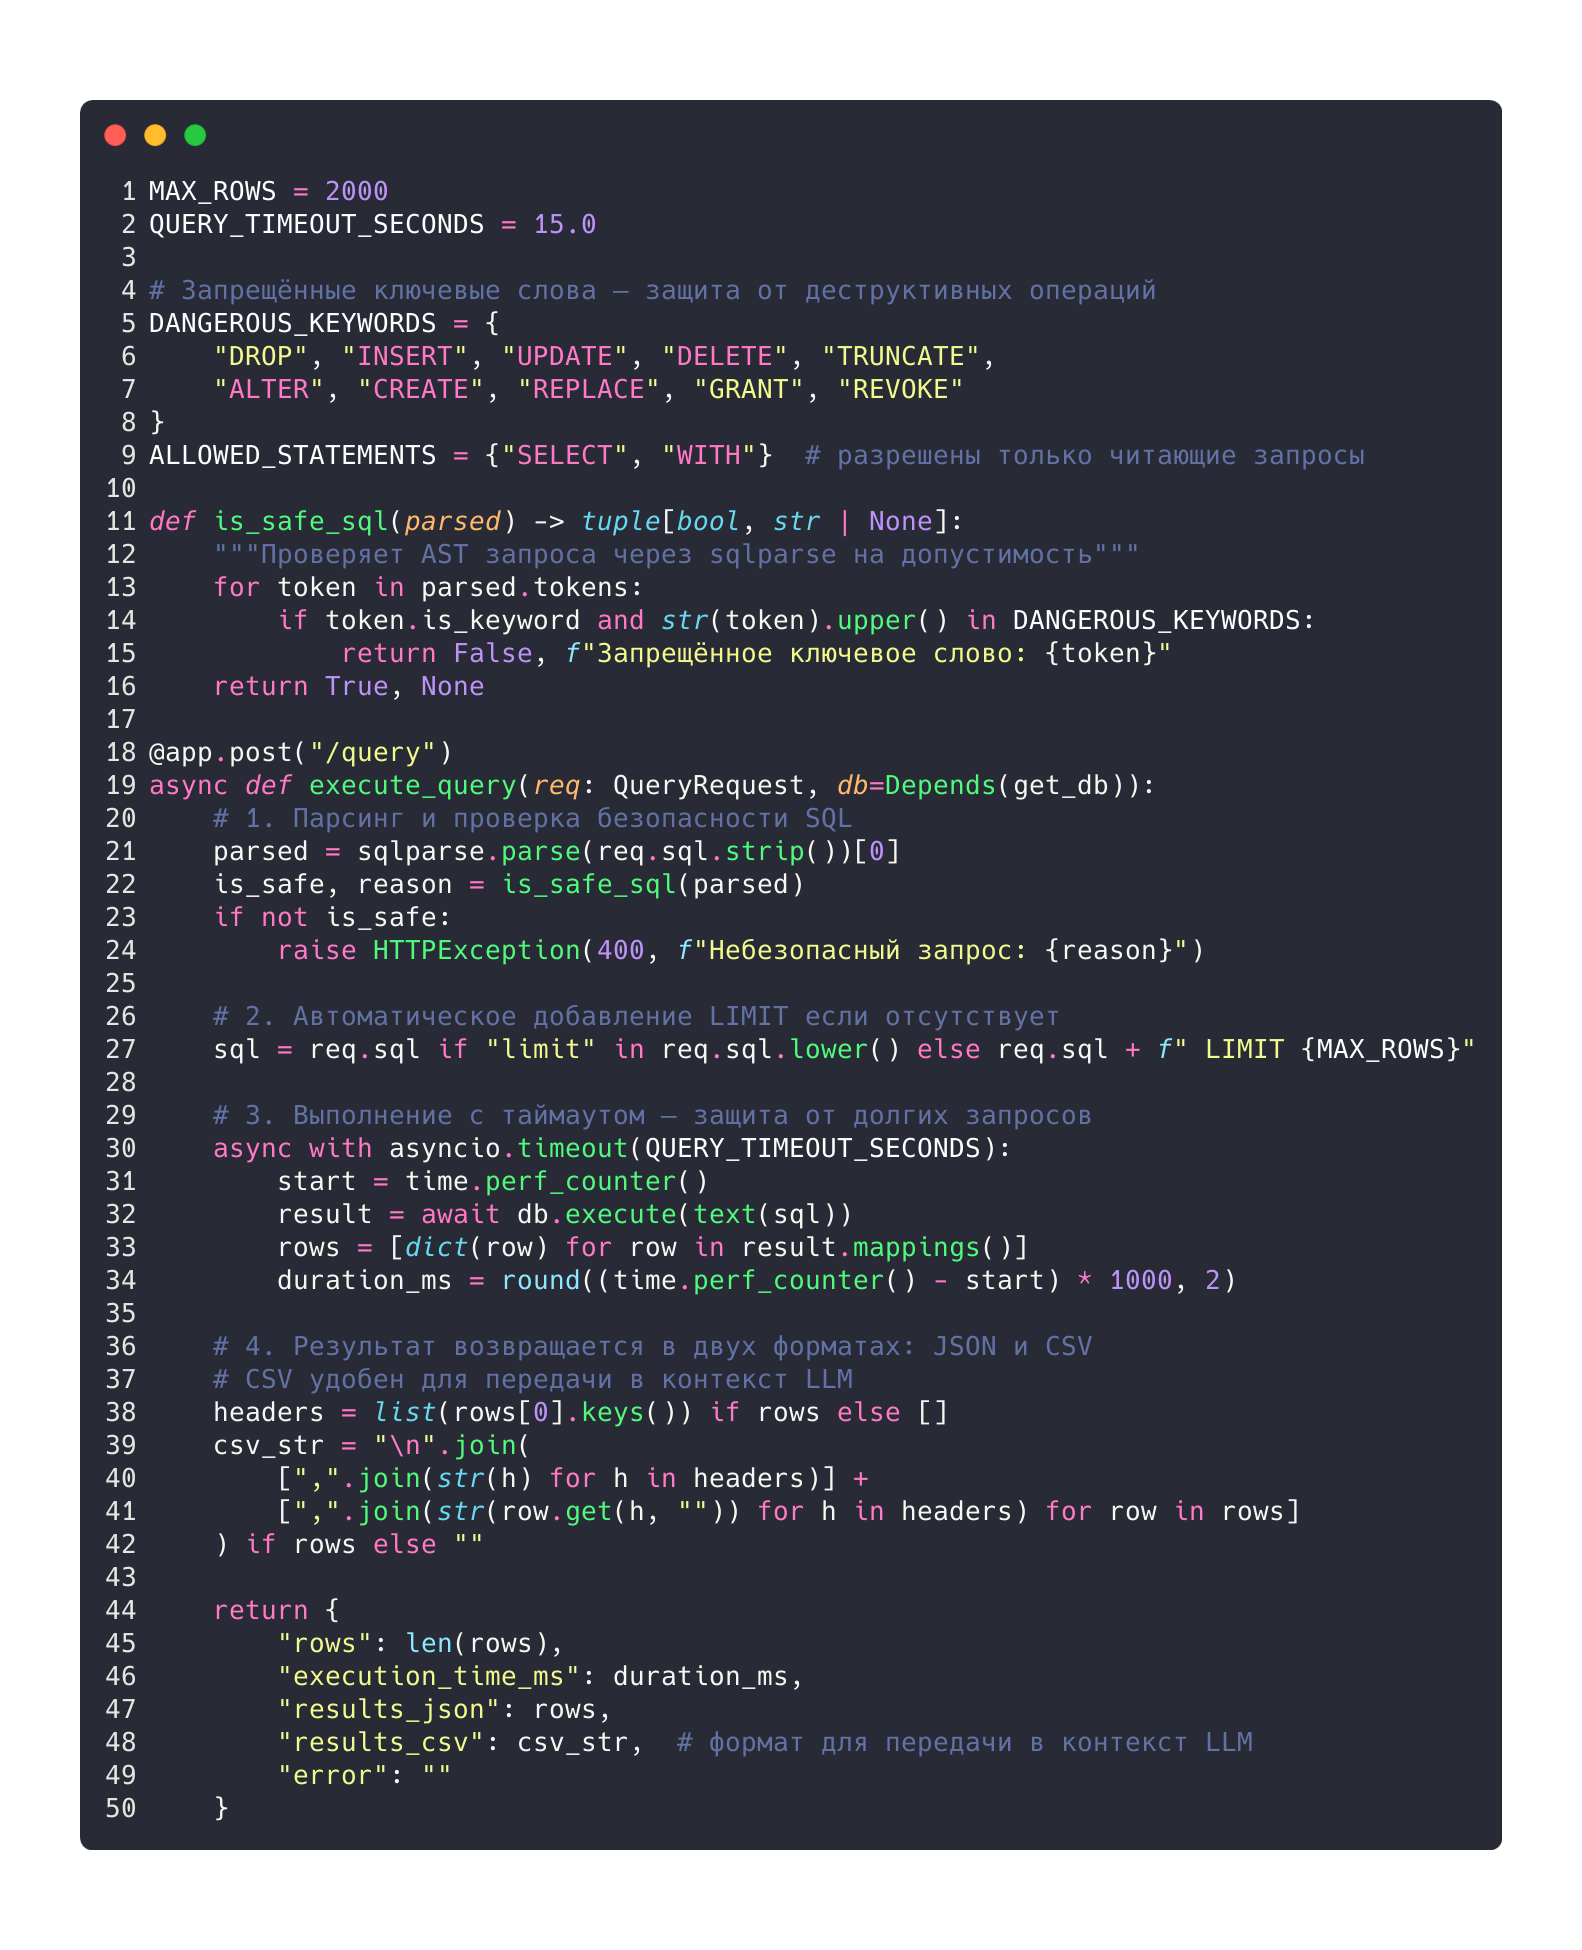
\includegraphics[width=\textwidth]{materials/codes/10.png}
    \caption{Многоуровневая проверка безопасности SQL-запросов в DB Connector Service}
    \label{code_10}
\end{figure}

Дополнительно сервис предоставляет эндпоинты для интроспекции схемы БД, используемые агентом при исправлении ошибок в SQL. Эти эндпоинты приведены на рисунке \ref{code_11}.

\begin{figure}[H]
    \centering
    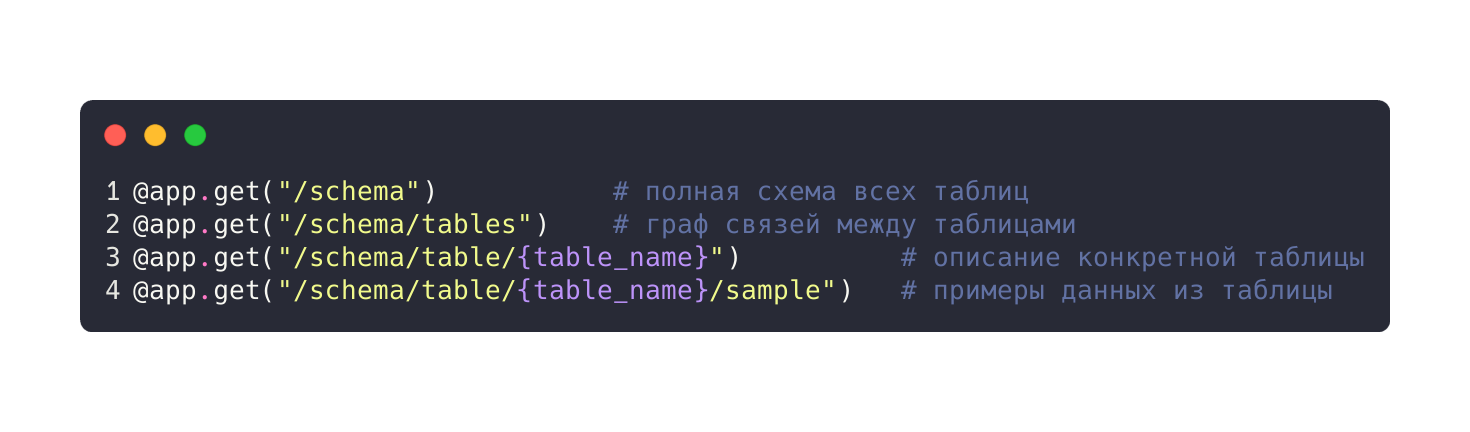
\includegraphics[width=\textwidth]{materials/codes/11.png}
    \caption{Эндпоинты DB Connector Service для получения схемы базы данных}
    \label{code_11}
\end{figure}

\subsection{Агентный модуль (Agent)}

\subsubsection{Структура состояния агента}

Состояние графа агента описывается через \texttt{TypedDict} и передаётся между вершинами графа. Оно содержит всю информацию, накапливаемую в процессе многошагового рассуждения: переписанный RAG-запрос, полученный контекст, сгенерированный SQL, результат его выполнения и вердикт критика. Структура состояния показана на рисунке \ref{code_12}.

\begin{figure}[H]
    \centering
    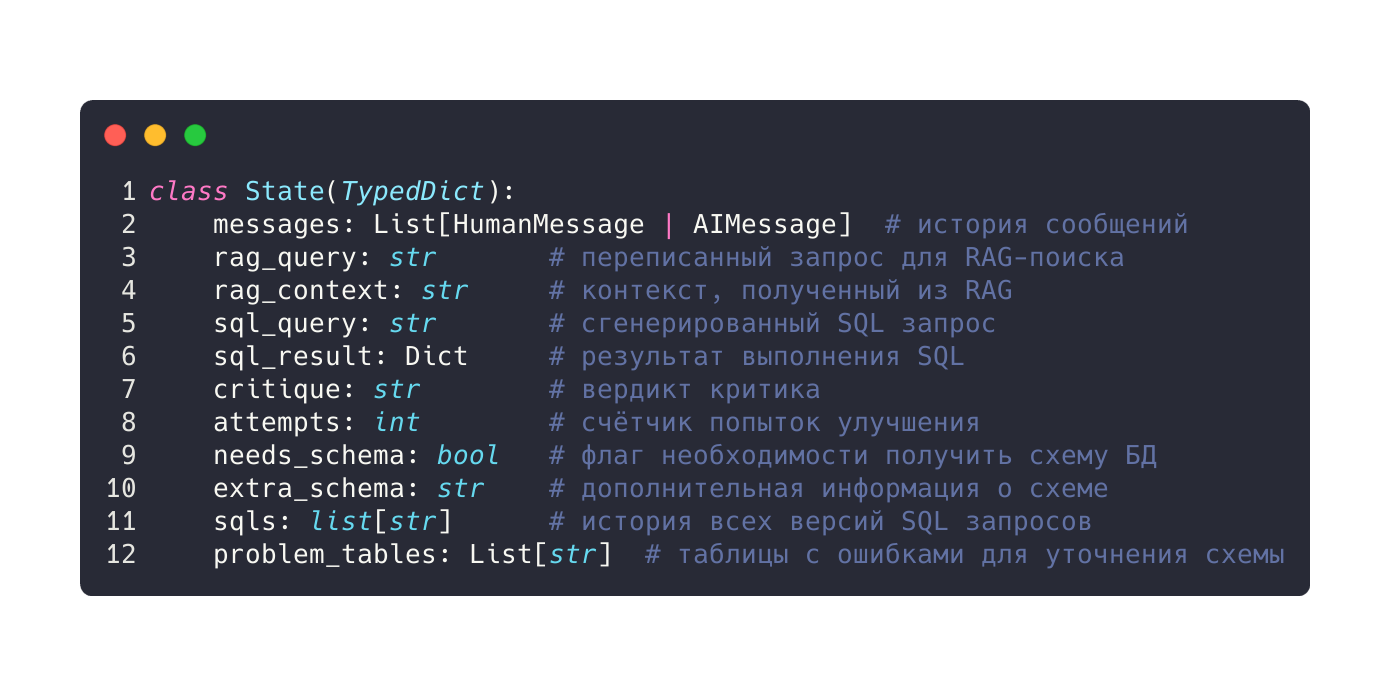
\includegraphics[width=\textwidth]{materials/codes/12.png}
    \caption{Определение состояния агента (\texttt{TypedDict}) для LangGraph}
    \label{code_12}
\end{figure}

\subsubsection{Граф агента (LangGraph)}

Агент реализован в виде ориентированного графа на основе \textbf{LangGraph}. Каждая вершина графа — это отдельный шаг обработки. После критики SQL граф принимает условное решение: завершить работу, запросить схему БД или улучшить SQL-запрос. Построение графа агента приведено на рисунке \ref{code_13}.

\begin{figure}[H]
    \centering
    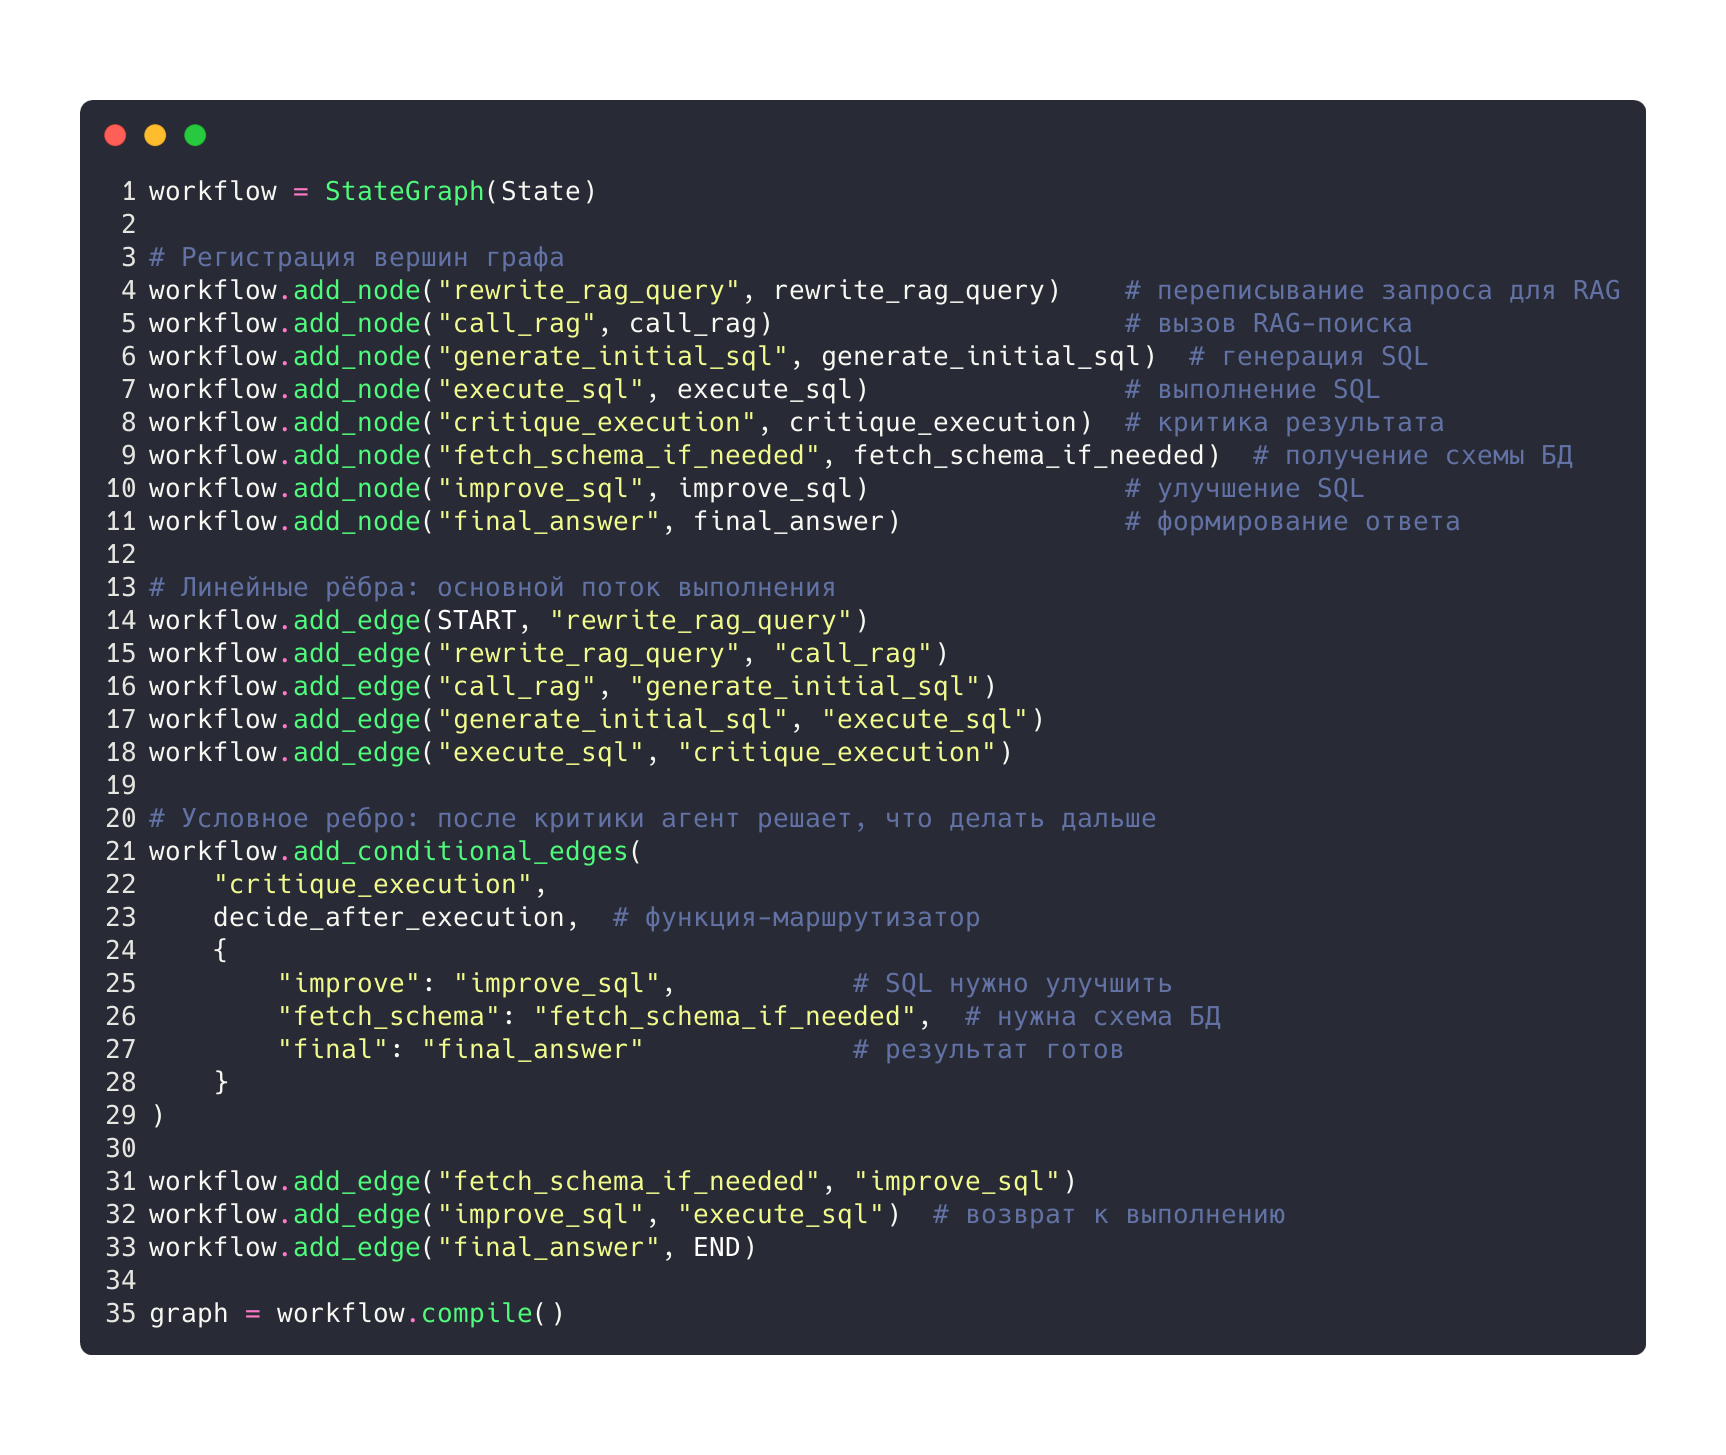
\includegraphics[width=\textwidth]{materials/codes/13.png}
    \caption{Построение графа агента с использованием LangGraph}
    \label{code_13}
\end{figure}

\subsubsection{Вершины графа: логика обработки}

\textbf{Переписывание запроса для RAG} — LLM адаптирует вопрос пользователя в поисковый запрос, обогащённый ключевыми словами для повышения точности семантического поиска. Реализация этой вершины показана на рисунке \ref{code_14}.

\begin{figure}[H]
    \centering
    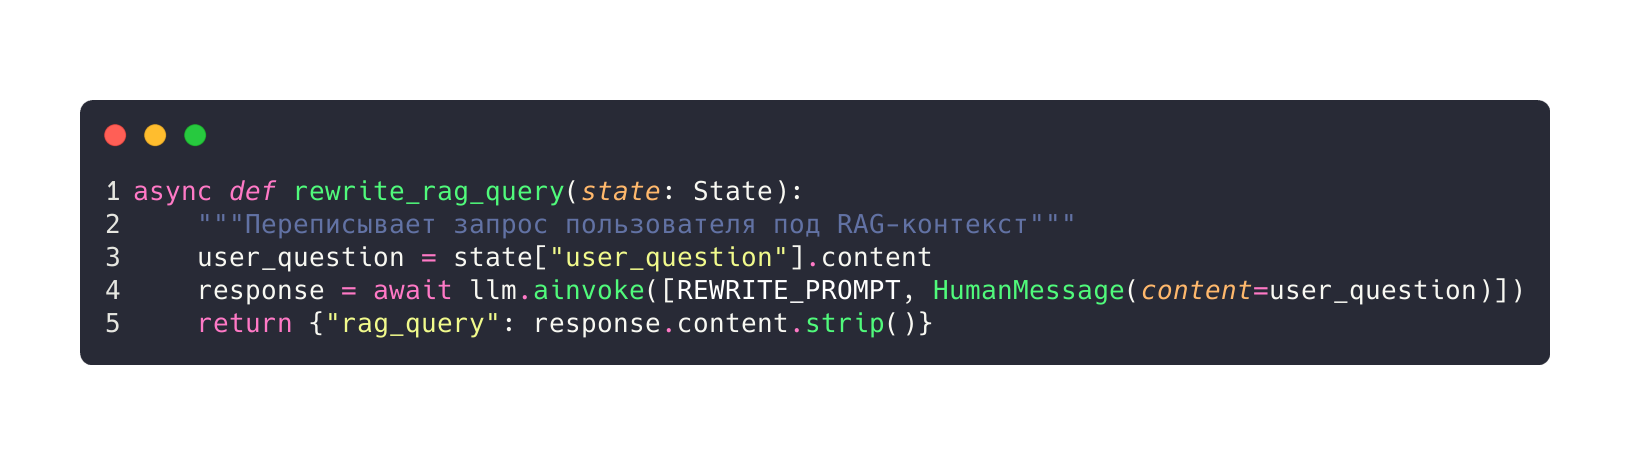
\includegraphics[width=\textwidth]{materials/codes/14.png}
    \caption{Вершина графа: переписывание пользовательского запроса для RAG}
    \label{code_14}
\end{figure}

\textbf{Вызов RAG-поиска} — вершина вызывает инструмент \texttt{rag\_search} и сохраняет полученный контекст в состоянии. Реализация вызова инструмента показана на рисунке \ref{code_15}.

\begin{figure}[H]
    \centering
    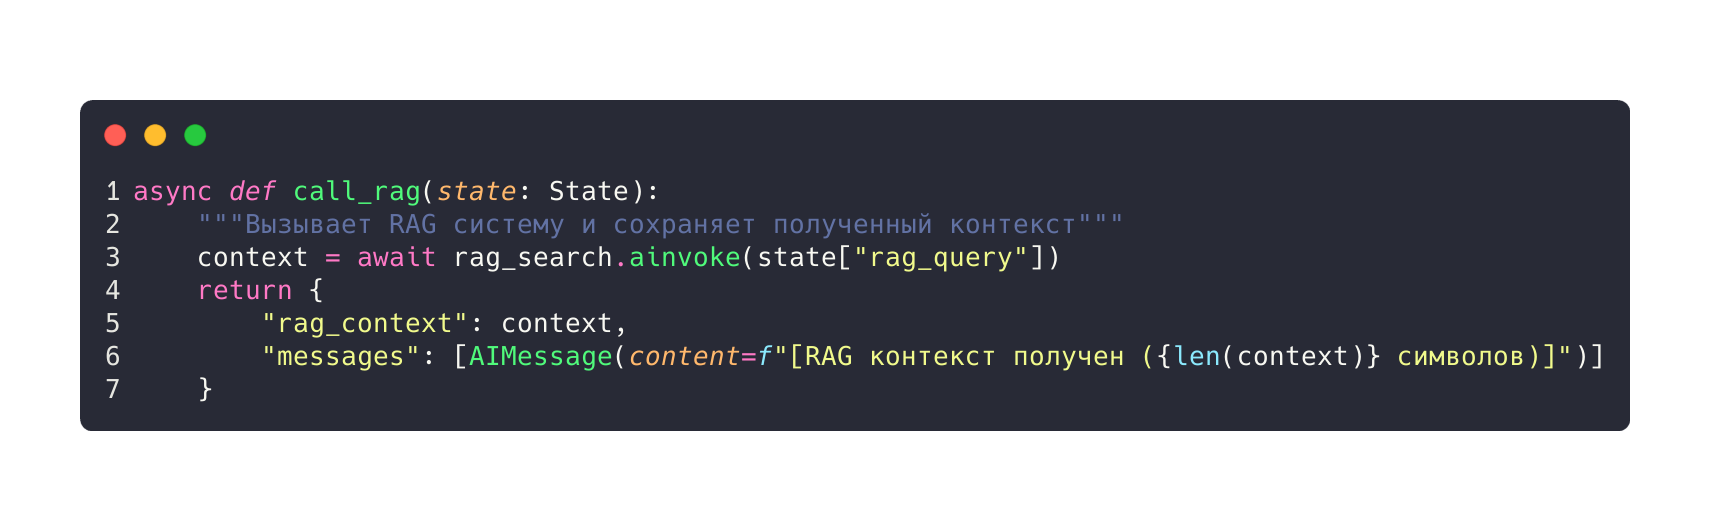
\includegraphics[width=\textwidth]{materials/codes/15.png}
    \caption{Вершина графа: вызов инструмента \texttt{rag\_search}}
    \label{code_15}
\end{figure}

\textbf{Генерация SQL} — на основе RAG-контекста LLM генерирует SQL-запрос. Реализация генерации SQL показана на рисунке \ref{code_16}.

\begin{figure}[H]
    \centering
    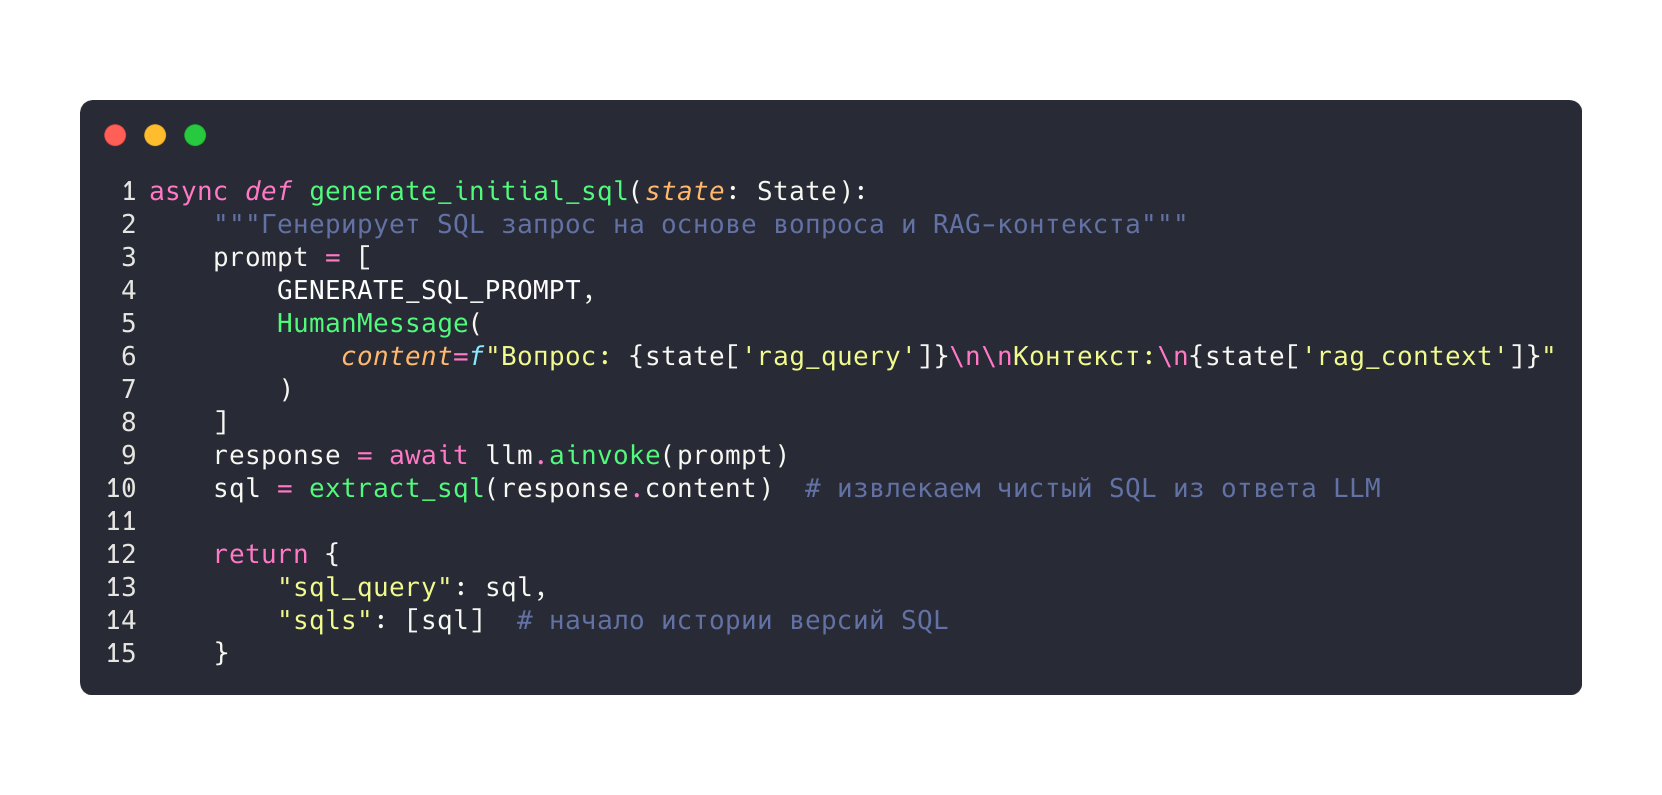
\includegraphics[width=\textwidth]{materials/codes/16.png}
    \caption{Вершина графа: генерация SQL-запроса на основе RAG-контекста}
    \label{code_16}
\end{figure}

\textbf{Выполнение SQL} — запрос отправляется в DB Connector Service и результат сохраняется в состоянии. Реализация выполнения запроса показана на рисунке \ref{code_17}.

\begin{figure}[H]
    \centering
    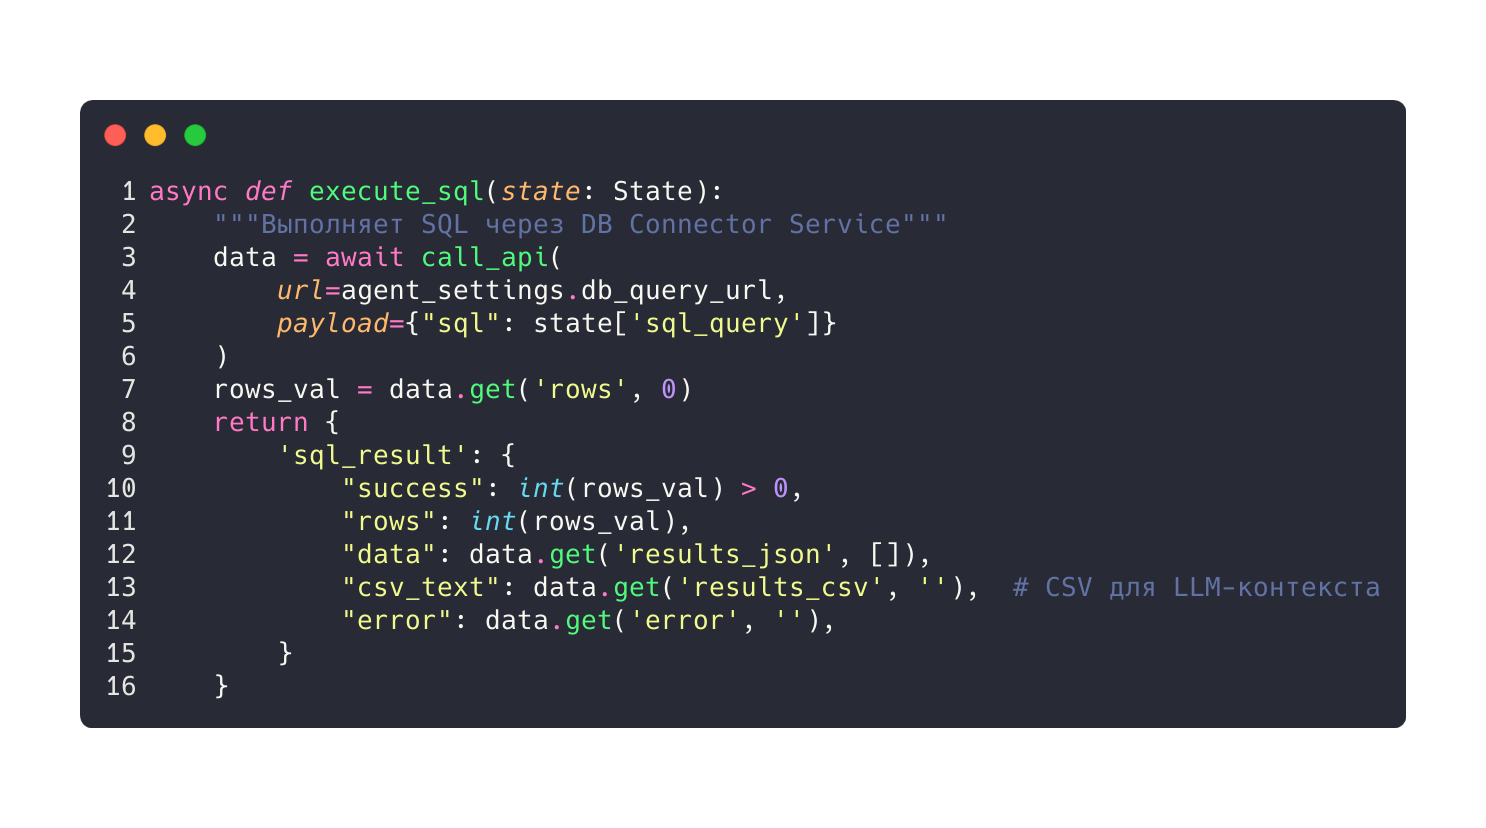
\includegraphics[width=\textwidth]{materials/codes/17.png}
    \caption{Вершина графа: выполнение SQL через DB Connector Service}
    \label{code_17}
\end{figure}

\textbf{Критика результата} — LLM анализирует результат выполнения SQL и выносит вердикт: принять результат или улучшать запрос, а также указывает на проблемные таблицы схемы. Реализация анализа результата показана на рисунке \ref{code_18}.

\begin{figure}[H]
    \centering
    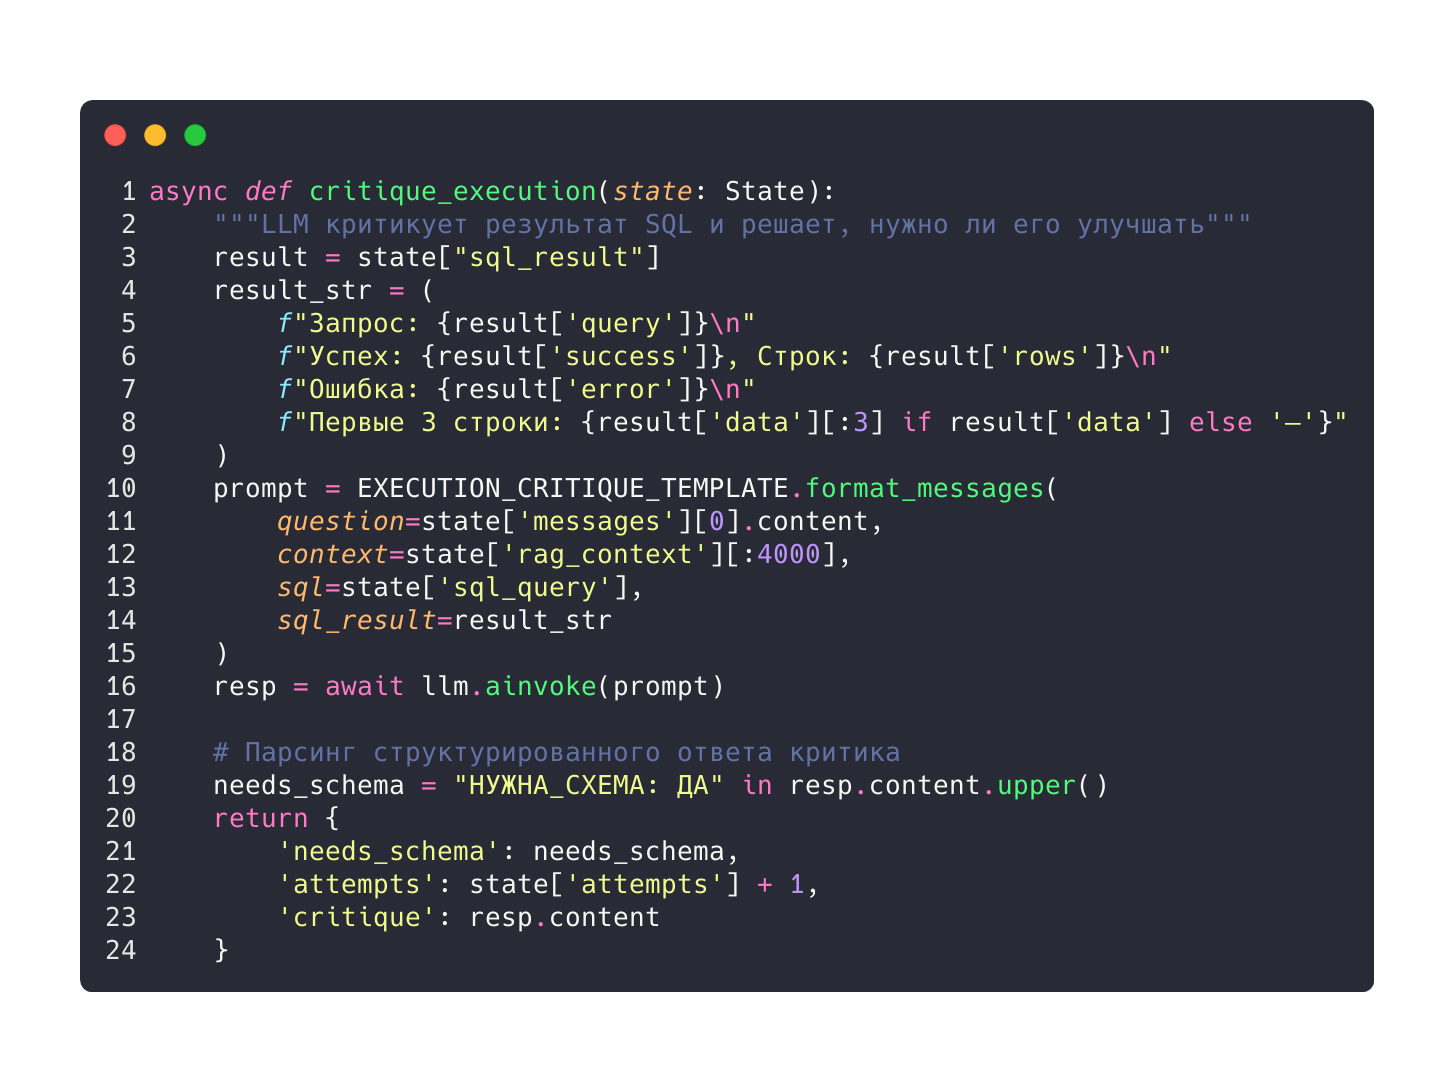
\includegraphics[width=\textwidth]{materials/codes/18.png}
    \caption{Вершина графа: анализ результата SQL и вынесение вердикта}
    \label{code_18}
\end{figure}

\textbf{Функция маршрутизации} — определяет следующий шаг на основе вердикта критика. Реализация условной маршрутизации показана на рисунке \ref{code_19}.

\begin{figure}[H]
    \centering
    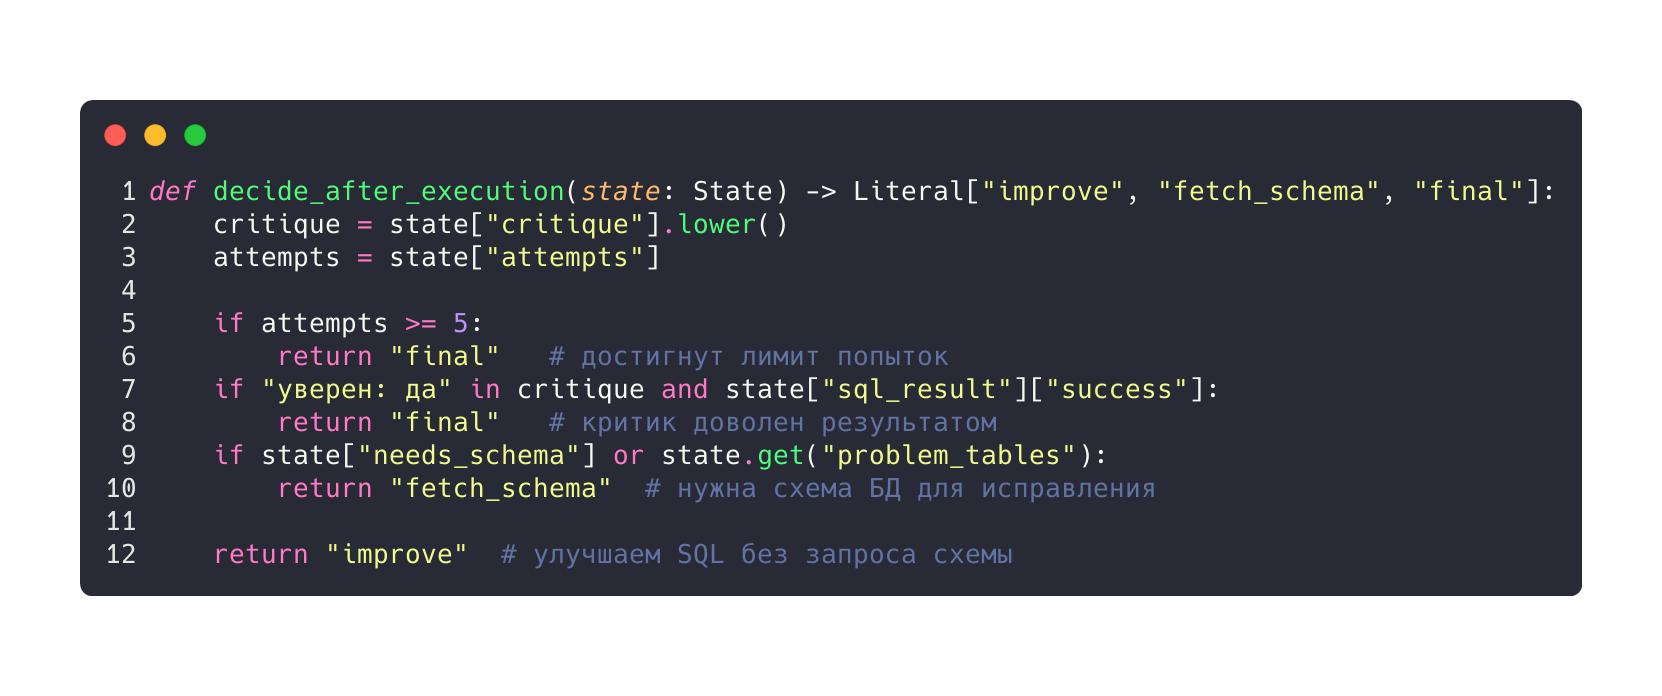
\includegraphics[width=\textwidth]{materials/codes/19.png}
    \caption{Функция условной маршрутизации на основе вердикта критика}
    \label{code_19}
\end{figure}

\textbf{Получение схемы БД} — если критик указал на проблемные таблицы, агент запрашивает их структуру и примеры данных у DB Connector Service. Реализация запроса схемы показана на рисунке \ref{code_20}.

\begin{figure}[H]
    \centering
    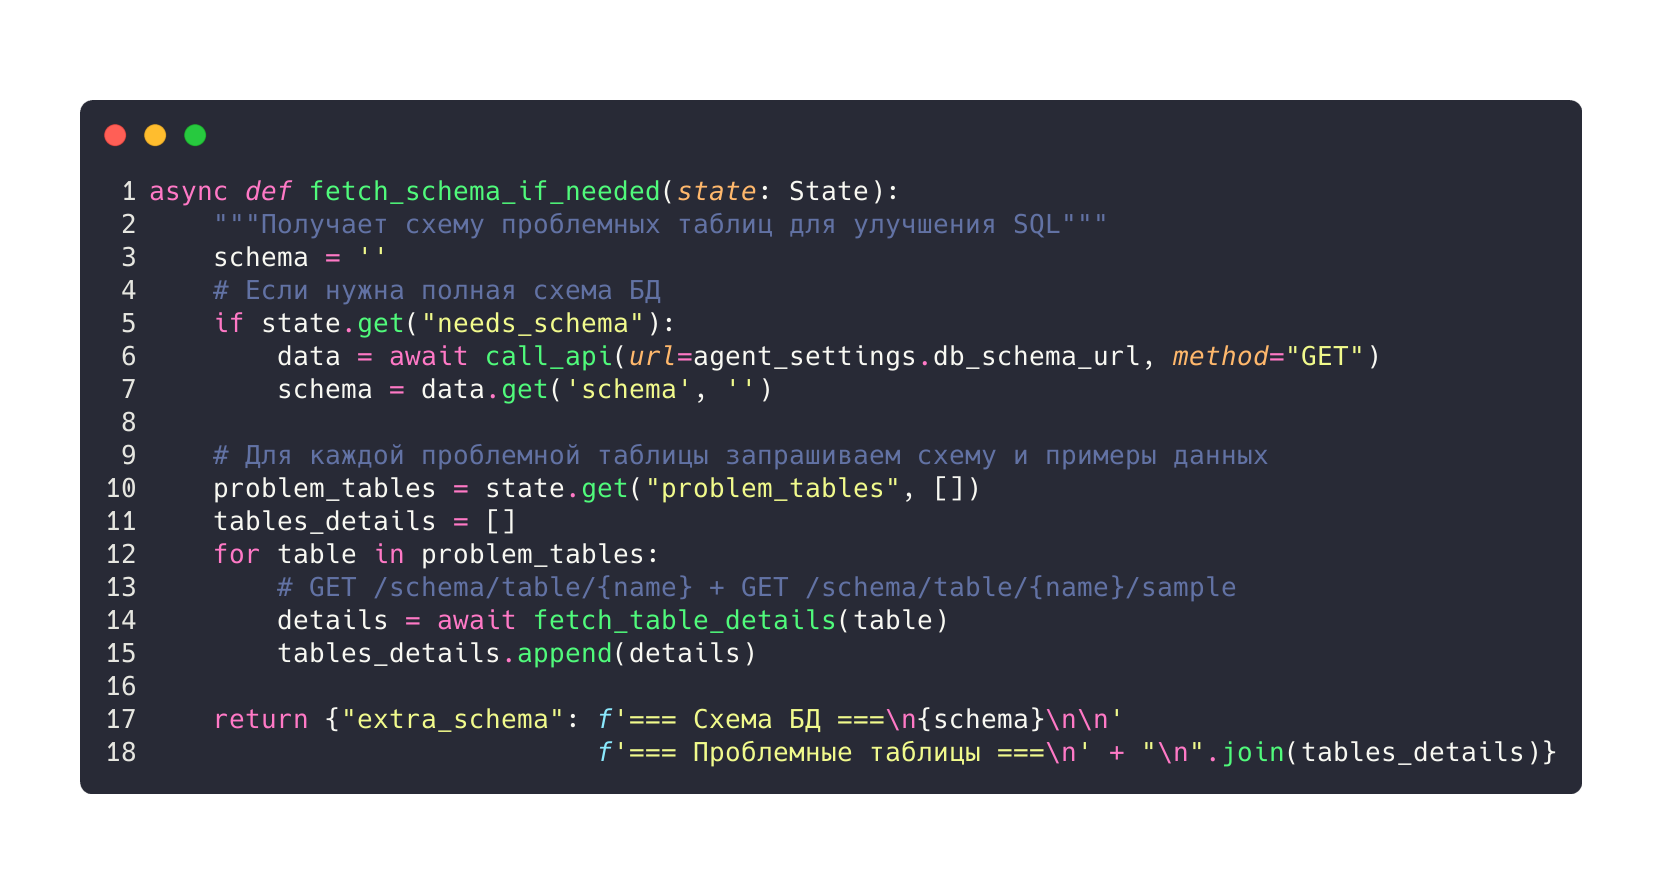
\includegraphics[width=\textwidth]{materials/codes/20.png}
    \caption{Вершина графа: запрос схемы проблемных таблиц}
    \label{code_20}
\end{figure}

\textbf{Улучшение SQL} — LLM переписывает SQL с учётом замечаний критика, истории предыдущих версий запроса и дополнительной схемы. Реализация улучшения SQL показана на рисунке \ref{code_21}.

\begin{figure}[H]
    \centering
    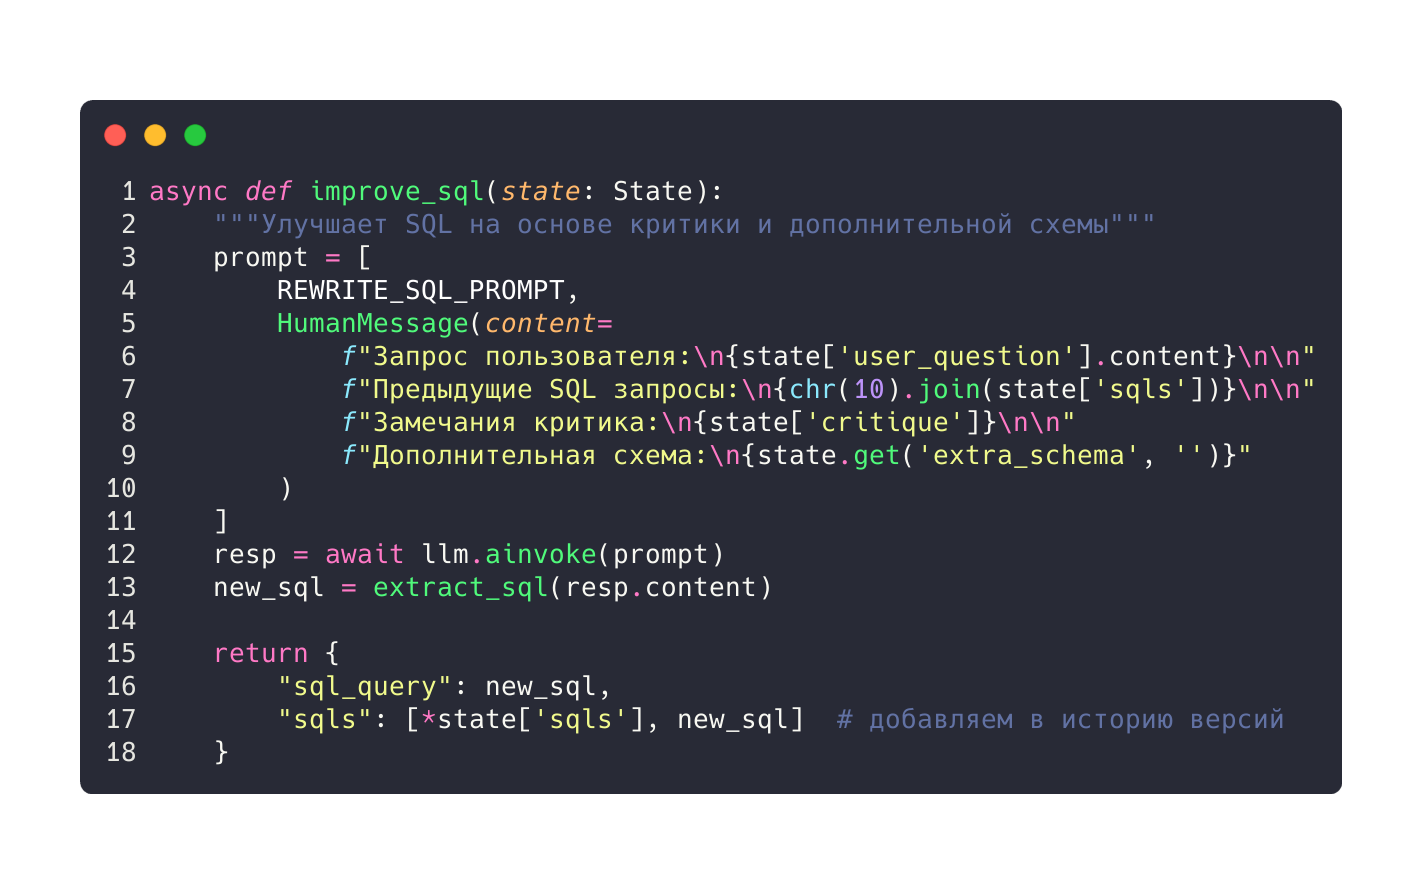
\includegraphics[width=\textwidth]{materials/codes/21.png}
    \caption{Вершина графа: улучшение SQL с учётом замечаний и схемы}
    \label{code_21}
\end{figure}

\subsubsection{Инструмент RAG-поиска агента}

Инструмент \texttt{rag\_search} оформлен как LangChain-tool с декоратором \texttt{@tool} и вызывается агентом в вершине \texttt{call\_rag}. Он обращается к Retrieval Pipeline Service и форматирует результаты с указанием источника и релевантности. Определение инструмента приведено на рисунке \ref{code_22}.

\begin{figure}[H]
    \centering
    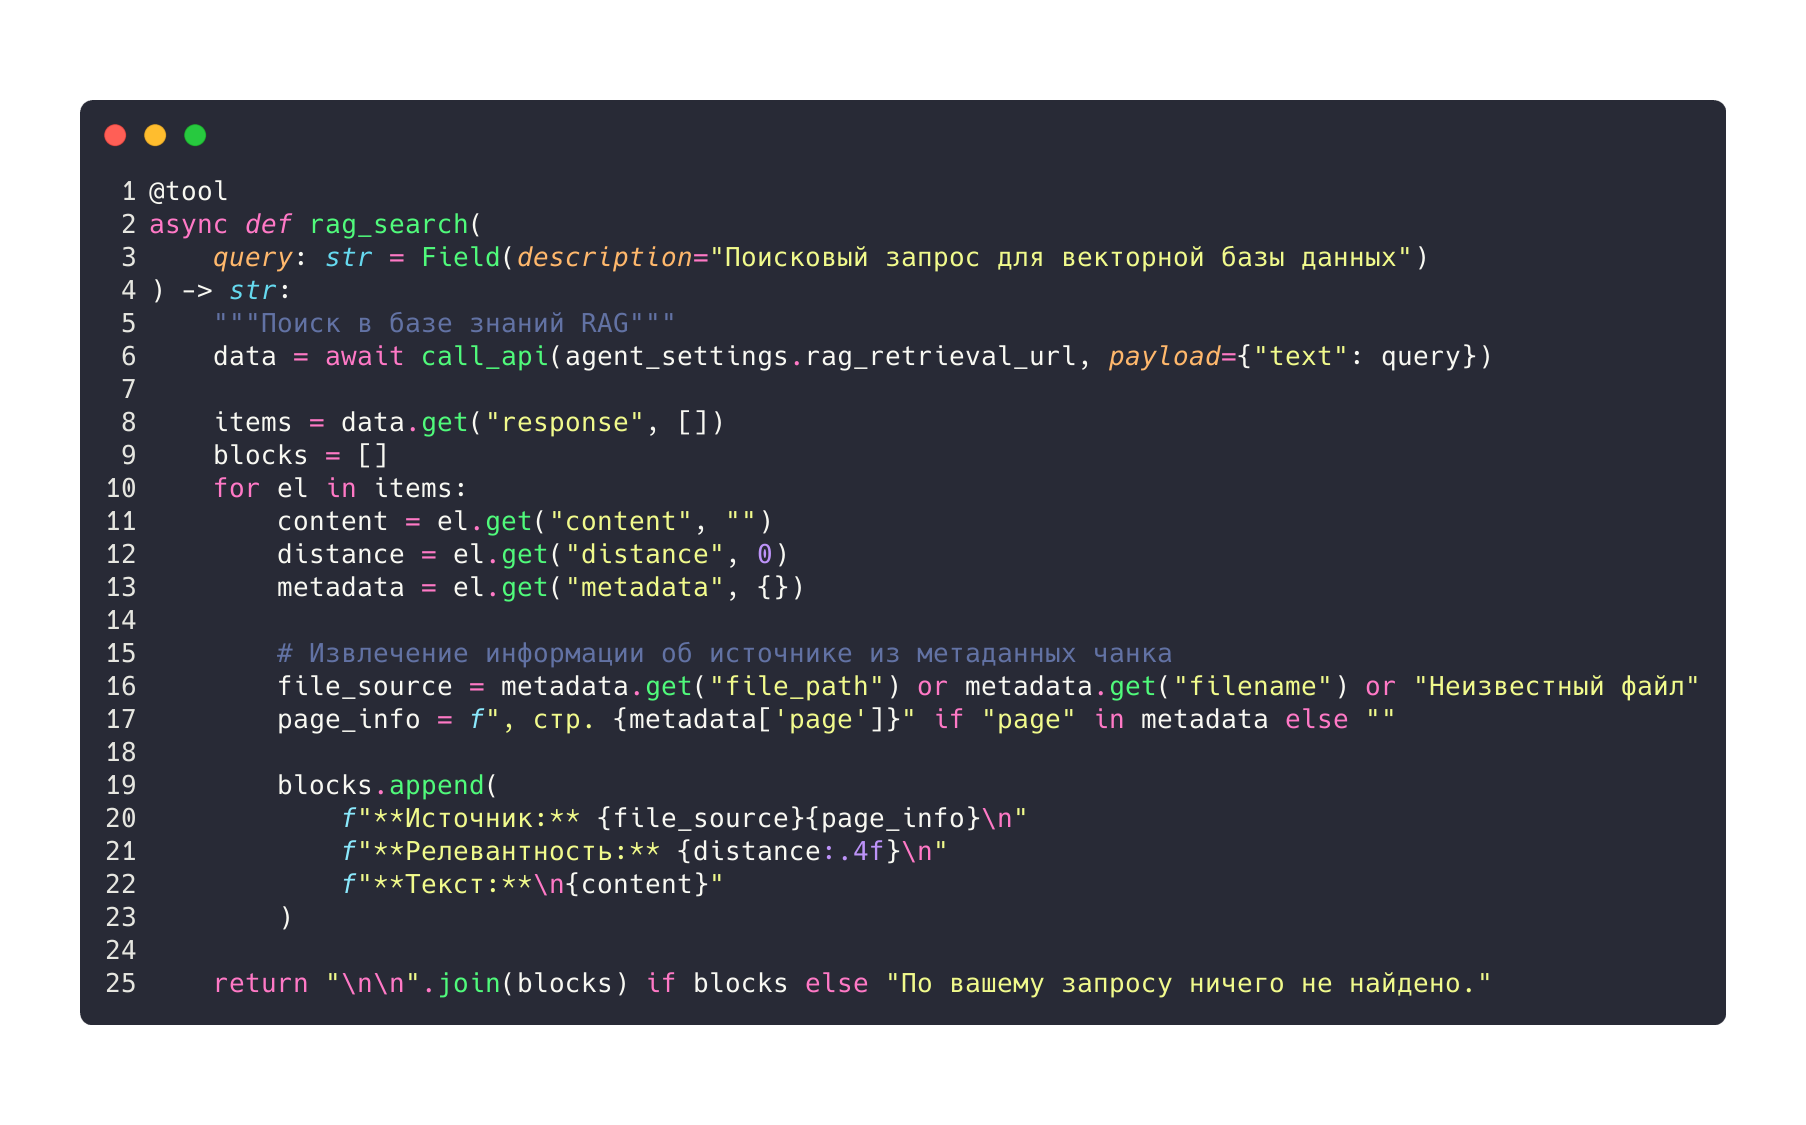
\includegraphics[width=\textwidth]{materials/codes/22.png}
    \caption{Определение инструмента \texttt{rag\_search} как LangChain Tool}
    \label{code_22}
\end{figure}

\subsubsection{Запуск агента}

Функция запуска агента и инвокации графа приведена на рисунке \ref{code_23}.

\begin{figure}[H]
    \centering
    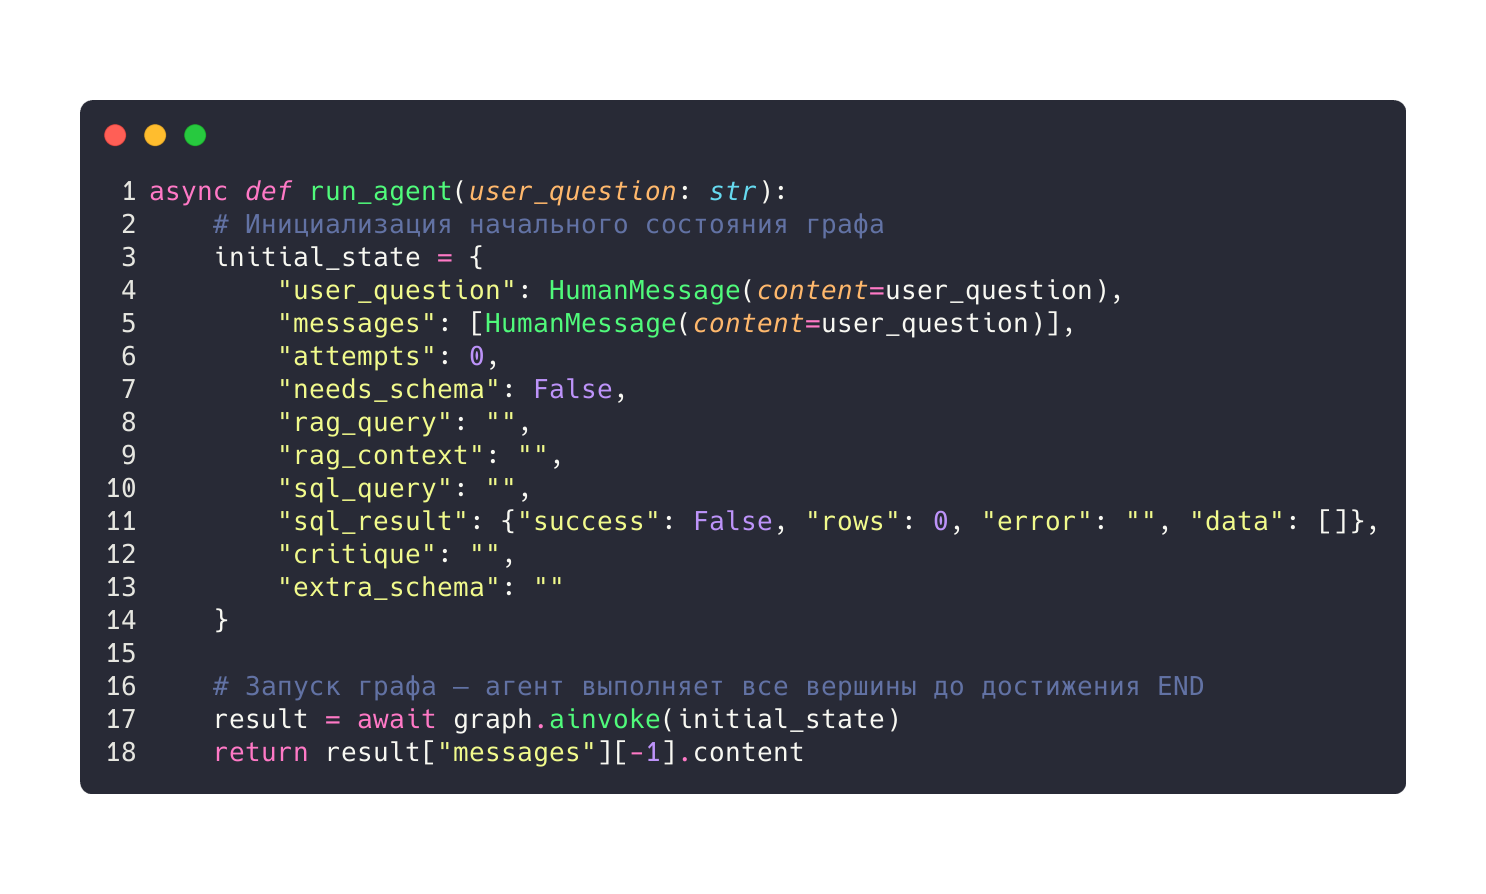
\includegraphics[width=\textwidth]{materials/codes/23.png}
    \caption{Функция запуска агента и инвокации графа}
    \label{code_23}
\end{figure}

\subsubsection{Универсальный клиент внешних API}

Все межсервисные вызовы в агенте выполняются через единую утилиту \texttt{call\_api}, которая поддерживает различные HTTP-методы и форматы ответа. Реализация универсального клиента показана на рисунке \ref{code_24}.

\begin{figure}[H]
    \centering
    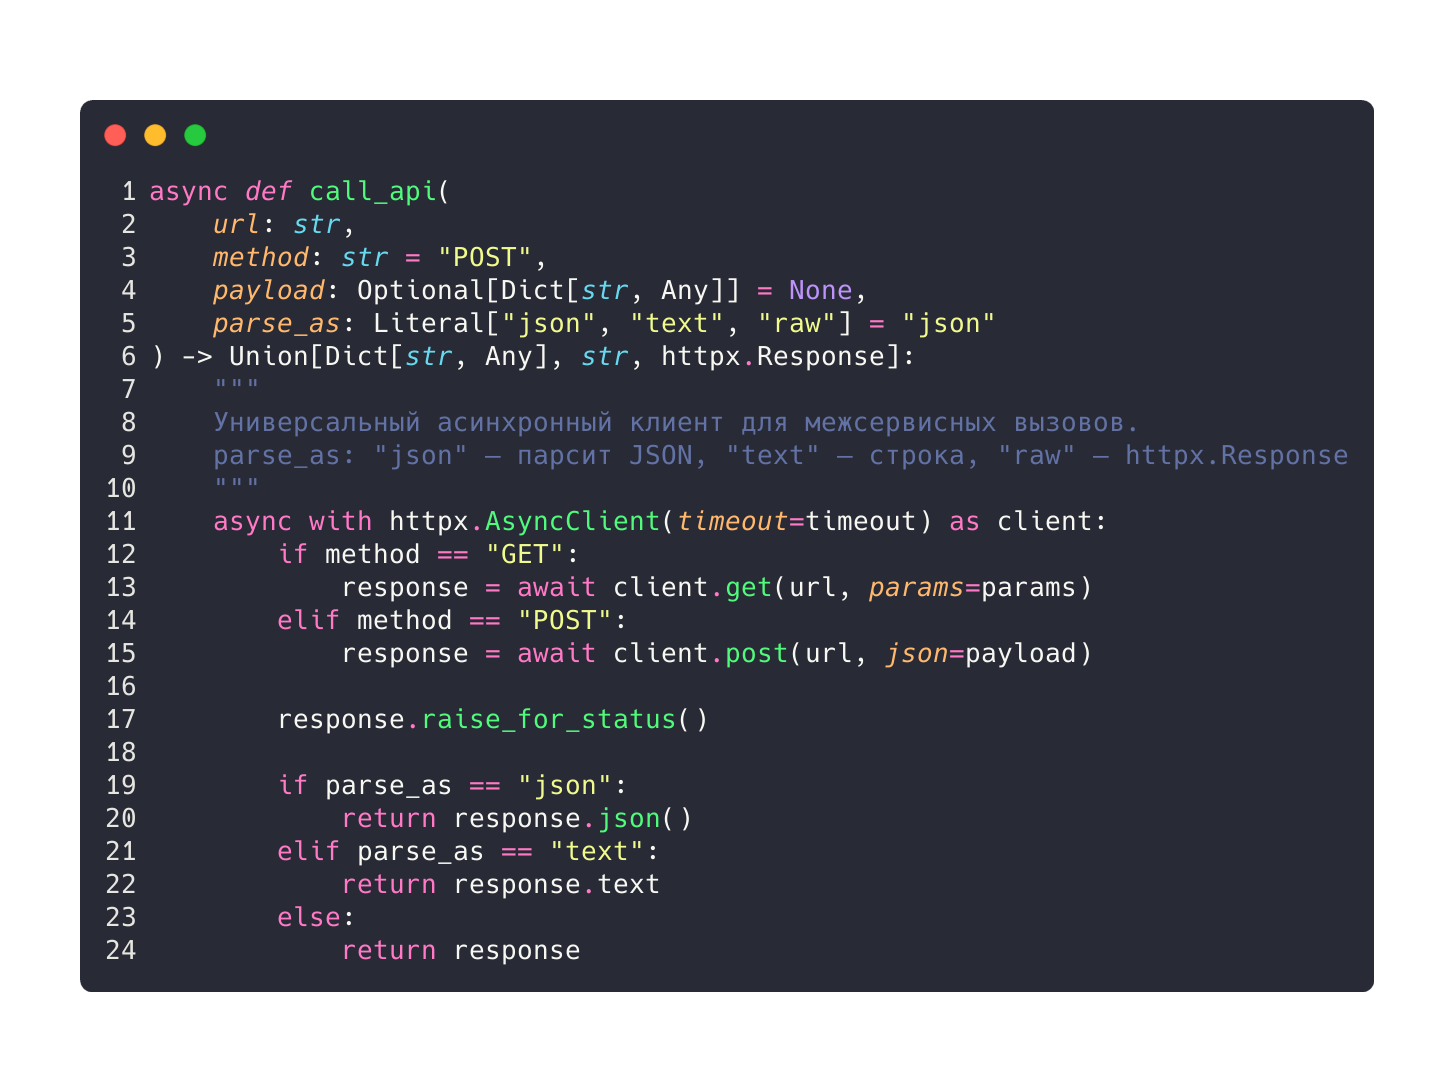
\includegraphics[width=\textwidth]{materials/codes/24.png}
    \caption{Единая утилита \texttt{call\_api} для межсервисных вызовов}
    \label{code_24}
\end{figure}
